\documentclass[11pt]{article} % For LaTeX2e
\usepackage{rldmsubmit,palatino}
\usepackage{graphicx}
\usepackage{verbatim} 
\usepackage{amsmath} % for 'bmatrix' environment
\usepackage{subcaption} % sub-figures with sub-labels
\usepackage{algpseudocode}

%%% Code Listing 
\usepackage{listings}
\usepackage{xcolor}

\definecolor{codegreen}{rgb}{0,0.6,0}
\definecolor{codegray}{rgb}{0.5,0.5,0.5}
\definecolor{codepurple}{rgb}{0.58,0,0.82}
\definecolor{backcolour}{rgb}{0.95,0.95,0.92}
\usepackage{listings}
\usepackage{tcolorbox}
\tcbuselibrary{listings}

\lstdefinestyle{mystyle}{
	backgroundcolor=\color{backcolour},   
	commentstyle=\color{codegreen},
	keywordstyle=\color{magenta},
	numberstyle=\tiny\color{codegray},
	stringstyle=\color{codepurple},
	basicstyle=\ttfamily\footnotesize,
	breakatwhitespace=false,         
	breaklines=true,                 
	captionpos=b,                    
	keepspaces=true,                 
	numbers=left,                    
	numbersep=5pt,                  
	showspaces=false,                
	showstringspaces=false,
	showtabs=false,                  
	tabsize=2
}
% sub-figures with sub-labels
\usepackage{subcaption}
\usepackage{float}
\usepackage[]{placeins}
\begin{comment}
   Applied Project: In the final report you should introduce the problem you solved 
   and the techniques used to solve the problem. If multiple algorithms were used 
   compare the performance of the different algorithms. If possible show how the 
   algorithms perform (accuracy and computation time) as the size of the problem 
   increases. If relevant show how your solutions methods perform if the model is 
   not accurately specified. Discuss any insights you have gained about your problem 
   as well as any insights about the best solution algorithm. Include a discussion 
   of potential shortcomings of your solution or problem formulation and how you 
   can improve these things. In addition, discuss possible extensions of your work.
\end{comment}
   

\title{Application of RL to Simulate Performance of an Unguided Hypersonic Glide Vehicle}


\author{
Justine John A Serdoncillo \\
Aerospace Engineering and Mechanics\\
University of Minnesota - Twin Cities\\
Minneapolis, MN  55414\\
\texttt{serdo004@umn.edu} \\
\And
Darryl Williams \\
Aerospace Engineering and Mechanics\\
University of Minnesota - Twin Cities\\
Minneapolis, MN  55414\\
\texttt{will7322@umn.edu} \\
}

% The \author macro works with any number of authors. There are two commands
% used to separate the names and addresses of multiple authors: \And and \AND.
%
% Using \And between authors leaves it to \LaTeX{} to determine where to break
% the lines. Using \AND forces a linebreak at that point. So, if \LaTeX{}
% puts 3 of 4 authors names on the first line, and the last on the second
% line, try using \AND instead of \And before the third author name.

\newcommand{\fix}{\marginpar{FIX}}
\newcommand{\new}{\marginpar{NEW}}

\begin{document}

\maketitle

\begin{comment}
\begin{abstract}

The \emph{title} should be a maximum of 100 characters. 

The \emph{abstract} should be a maximum of 2000 characters of text,
including spaces (no figure is allowed). You will be asked to copy
this into a text-only box; and it will appear as such in the
conference booklet. Use 11~point type, with a vertical spacing of
12~points.  The word \textbf{Abstract} must be centered, bold, and in
point size 12. Two line spaces precede the abstract.
Our project aims to simulate the performance of a high-speed aircraft using simplified physics.
We have chosen an unguided hypersonic glide vehicle (HGV) as the exemplar case. The primary
objective is to develop a control policy that ensures the vehicle maintains a straight heading. Typ-
ically, achieving this would involve approximating derivatives or deriving analytical expressions
for application in a feedback controller.
However, we are taking a different approach by utilizing reinforcement learning (RL) to create
an optimal policy for maintaining the heading angle.
\end{abstract}

\keywords{
Q-Learning, Neural Networks, Glide Vehicles
}

\acknowledgements{We are deeply indebted to Google DeepMind and
the Weinberg Institute for Cognitive Science for
their generous support of RLDM2017.}  

\startmain % to start the main 1-4 pages of the submission.
\section{Submission of papers to RLDM}

RLDM requires electronic submissions.  This year's electronic
submission site is   
\begin{center}
   https://cmt3.research.microsoft.com/RLDM2017/
\end{center}

Please read the instructions below, and follow them faithfully. Note
that there is also a template \verb+rldm.rtf+ for Microsoft Word,
which is available from the website below.
\subsection{Style}

Papers to be submitted to RLDM must be prepared according to the
instructions presented here. Papers consist of a \emph{title}, which
has a maximum of 100 characters, an \emph{abstract}, which is a
maximum of 2000 characters, up to five key words, and an
\emph{extended abstract}, which starts on the second page, and can be
between one and four pages. Figures and references should be included
in the latter.

Authors preferring \LaTeX{} are requested to use the RLDM \LaTeX{}
style files obtainable at the RLDM website at
\begin{center}
   http://www.rldm.org/
\end{center}
The file \verb+rldm.pdf+ contains these instructions and illustrates
the various formatting requirements your RLDM paper must
satisfy. There is a \LaTeX{} style file called \verb+rldmsubmit.sty+,
and a \LaTeX{} file \verb+rldm.tex+, which may be used as a ``shell''
for writing your paper. All you have to do is replace the author,
title, abstract, keywords, acknowledgements and text of the paper with
your own. The file
\verb+rldm.rtf+ is provided as an equivalent shell for Microsoft Word users. 

\section{General formatting instructions}
\label{gen_inst}

The paper size for RLDM is ``US Letter'' (rather than ``A4''). Margins
are 1.5cm around all sides. Use 11~point type with a vertical spacing
of 12~points. Palatino is the preferred typeface throughout.
Paragraphs are separated by 1/2~line space, with no indentation.

Paper title is 17~point, initial caps/lower case, bold, centered between
2~horizontal rules. Top rule is 4~points thick and bottom rule is 1~point
thick. Allow 0.6cm space above and below title to rules. 

The lead author's name is to be listed first (left-most), and
the co-authors' names (if different address) are set to follow. If
there is only one co-author, list both author and co-author side by side.

\section{Preparing PostScript or PDF files}

Please prepare PostScript or PDF files with paper size ``US Letter''.
The -t letter option on dvips will produce US Letter files.
\end{comment}

\begin{abstract}. 
   
   In this paper, we present a novel approach for simulating and controlling a 
   high-speed aircraft using simplified physics and reinforcement learning (RL).
   We focus on the case of an unguided hypersonic glide vehicle (HGV), 
   which is a challenging and relevant problem for aerospace engineering.
   Our goal is to design a control policy that can keep the vehicle on a straight heading, 
   without relying on analytical expressions or numerical approximations of the dynamics. 
   To achieve this, we use neural networks to model the continuous state space 
   and the action space of the system, and apply RL algorithms to learn the optimal policy from data. 
   We compare our approach with conventional methods and demonstrate its effectiveness 
   and robustness in various scenarios. Our results show that RL can offer a 
   viable and efficient alternative for controlling high-speed aircraft.
\end{abstract}
   
\keywords{Q-Learning, Neural Networks, Glide Vehicles}

\section{Problem Introduction}
Hypersonic glide vehicles (HGVs) are capable of maneuvering within earth's atmosphere as they glide at high-speeds
in excess of Mach 5. As a result of their speed, HGVs are able to travel several thousand kilometers within a short
amount of time. Their ability to achieve long distances in short time frames and their use of aerodynamic forces for
maneuvering have made them a subject of extensive research, particularly for defense applications.
A typical trajectory for HGVs involves a boost phase that brings the vehicle high in the atmosphere, a reentry phase,
and a glide phase at speeds of Mach 5-20. 

In this paper we use a deep Q-learning approach with experience reply to perform guidance on an HGV during its glide 
phase. In the implemented framework, an aerodynamic code is integrated into the equation of motion over a 
non-rotating spherical Earth:

\begin{equation}
   \frac{\partial}{\partial t}
   \begin{bmatrix}
       \gamma \\
       V \\
       x \\
       h 
   \end{bmatrix} =
   \begin{bmatrix}
       \frac{1}{V} \left[\frac{L}{m}+g \cos(\gamma)-\frac{V^2}{R} \cos(\gamma)\right] \\
       \frac{D}{m}+ g\sin(\gamma)\\
       -V\cos(\gamma) \\
       -V\sin(\gamma)
   \end{bmatrix} \, .
   \label{eqn:EOM}
\end{equation}

We then use an optimal policy $\pi^*$, to preform guidance on the HGV initial conditions of 60 km in altitude traveling
at 6 km/s. Newtonian Aerodynamic (NA) was used as a lower-fidelity tool to compute the aerodynamic forces acting on the
HGV. This approximate method is much cheaper than computational fluid dynamics enabling rapid exploration of the simulated
environment but for lower levels of accuracy. Newtonian aerodynamics assumes tangential velocities are unchanged, while the
normal velocity results in aerodynamic forces acting on the vehicle as shown in figure \ref{fig:NA}. 
\begin{figure}[H]
   \centering
     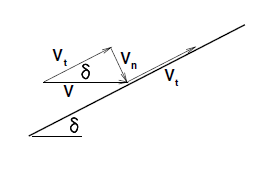
\includegraphics[width=0.5\textwidth]{images/NA.png}
   \caption{Illustration of tangential and normal velocities on surface.}
   \label{fig:NA}
\end{figure}
This approximation is more accurate as speeds are increased into higher mach numbers. The algorithm to compute forces over
a tessellated surface is described in the NA Procedure below.

\begin{algorithmic}
   \State $N =$ number of triangles elements
   \Procedure{NA}{$\alpha$} %\Comment{The g.c.d. of a and b}
       \State $i \gets 1$
   \State $\hat{v} =\{\cos(\alpha),sin(\alpha),0\} $
   \State Forces =$\{0,0,0\} $
   \While{$i \leq N$}
   \If{$(\hat{v} \cdot \hat{n}_i) < 0$}
       \State  ${cp}_i = 2 \left(\hat{v} \cdot \hat{n}_i\right)^2$
   \Else
       \State  ${cp}_i = 0$ \Comment{Flow is hidden from velocity vector}
   \EndIf
   \State  $P_i=({cp}_i \cdot q)+P_{\infty}$
   \State  $F = F + (P_i \cdot A_i)\cdot(-\hat{n}_i) $\Comment{$A_i$  computed from cross product}
   \State $i \gets i+1$
   \EndWhile
   \State  $D=F(2)\sin(\alpha)+F(1)\cos(\alpha)$
   \State  $L=F(2)\cos(\alpha)-F(1)\sin(\alpha)$
   \EndProcedure
\end{algorithmic}

We then use the aerodynamic forces(L,D) to compute the derivatives in Equation \ref{eqn:EOM}. Time was integrated using the
4-th order Runga-Kutta method with a fixed time-step of $\Delta t = 1$ seconds as the time discretization. 

\section{Methodology}
   \subsection{Simulation Environment}
   Our policy $\pi$(a = $\alpha|s$), when given a state, selects an angle of attack ($\alpha$) such that forces on the
   vehicle, lift ($L$) and drag ($D$), are modulated. With these forces, we can then integrate the equation of motion
   for a fixed $\delta t$ to arrive at out new state. We note that the simulated environment is not representative
   of actual flight. Rather, this model for system dynamics is sought as a proof of concept and to have tractable 
   training times of the algorithm used. The relative disparity between system dynamics comparing a computational  
   fluid dynamics approach to NA is shown in Figure \ref{fig:compare}.
   \begin{figure}[H]
      \centering
        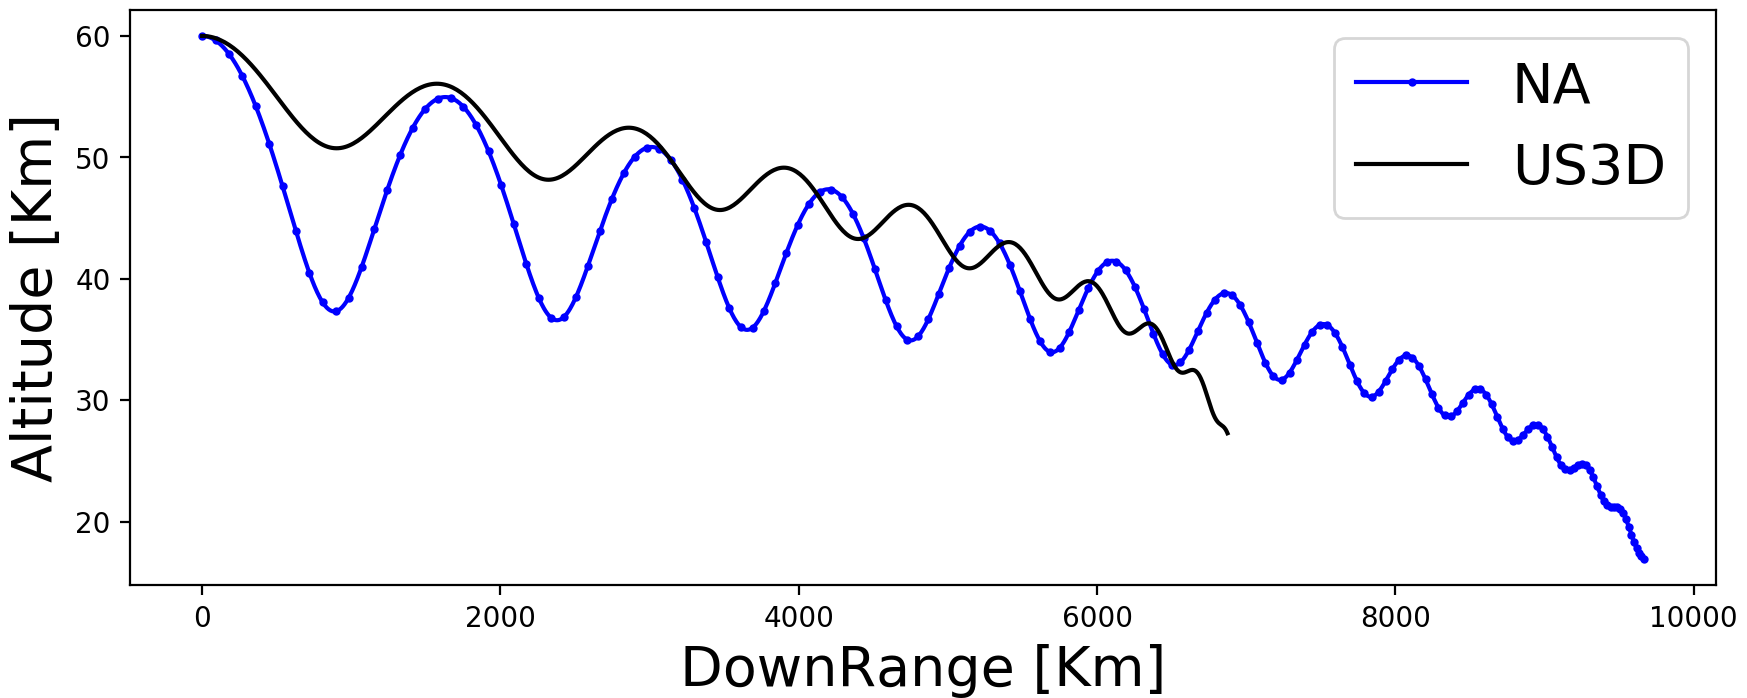
\includegraphics[width=0.65\textwidth]{images/compare_alt.png}
        \caption{Comparison between full trajectory using US3D (CFD) and NA. }
        \label{fig:compare}

   \end{figure}
\subsection{Markov Decision Process model}
We implemented an epsilon greedy approach for exploration. Modeled as an episodic problem that terminated once the
altitude went below 1 km or velocity decreased below 1 km/s. A summary of major hyperparameters and state space below:
\begin{itemize}
   \item State Space: $\gamma$, $h$,$V$
   \item Action: $\alpha$
   \item $\epsilon_{i+1} = 1+ \log(\epsilon_i/(0.6*n))$
   \item  Problem: Episodic with gamma = 0.9 
   \item Rewards: $- \gamma^2$ + d
\end{itemize}


\subsection{Neural Networks for continuous State Space RL}
Artificial neural networks have been used for extensively for nonlinear function approximation. 
It characterized by applying a linear model to a feature vector then applying a non-linear mapping.
This neural networks are often convoluted within each other its to have several instances of linear and non-linear 
mappings applied to them. This type of neural network architecture is known as a deep neural network. For the 
implemented method we decided on a neural network composed of two 24 neuron hidden layers, The non-linear activation
decided was the use of the rectified linear unit. 

In our case, we are using a deep Q-learning methodology by using an input tuple of the state, action, new state, and the reward. Our 
compute time was broken into the following:
\begin{itemize}

   \item Exploration: first 25\%
   \begin{itemize}
      \item choosing random actions to explore the state transitions
      \item store [state, action, state prime, reward] for each combination
   \end{itemize}
   
   \item Training: second 65\%
   \begin{itemize}
      \item reduction of epsilon to reduce exploration
      \item trains using stored memory
      \item input is the state and action, output is the next state and reward
   \end{itemize}
   
   \item Testing: last 10\%
   \begin{itemize}
      \item test neural net by running on new intial conditions and trajectories
   \end{itemize}
   
   \end{itemize}
   
   The figure below shows the algorithm that we based our neural network on. The code for the environment and neural network as seen in the appendices below.
   
   \begin{figure}[H]
      \centering
        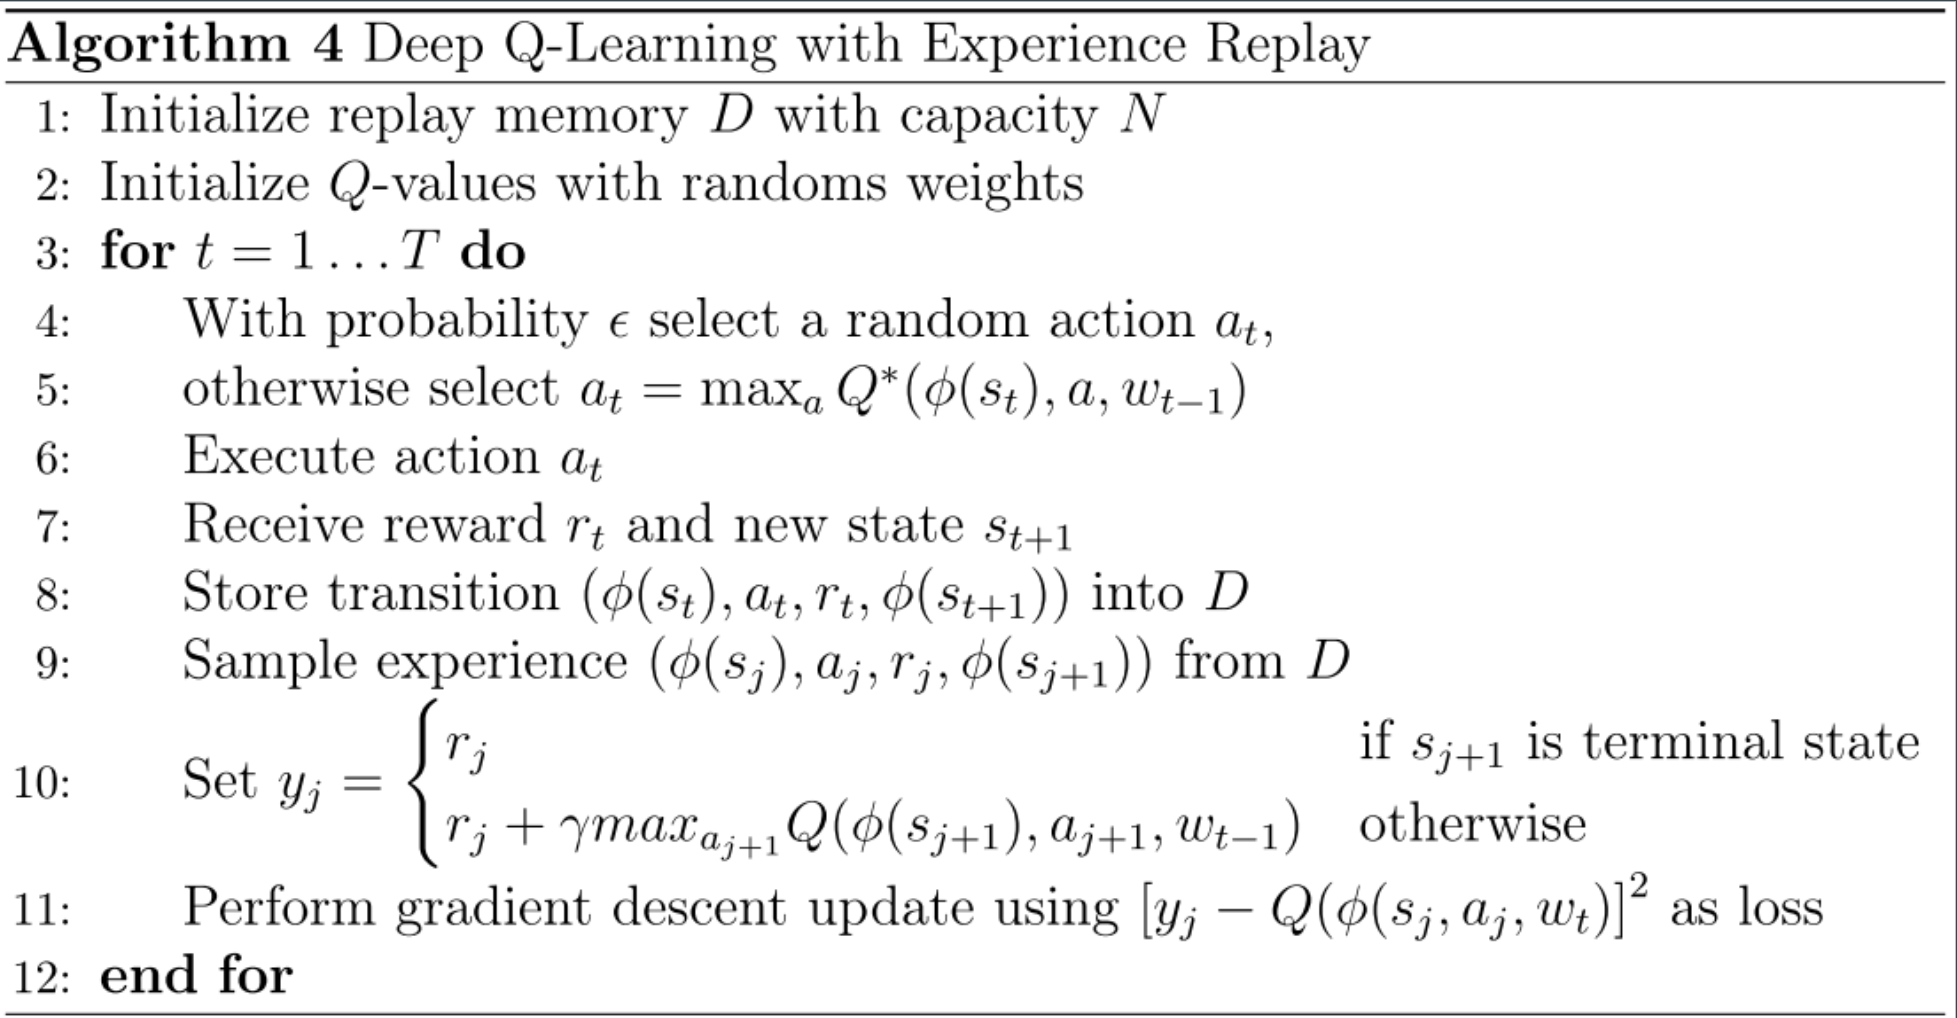
\includegraphics[width=0.65\textwidth]{images/alg.png}
        \caption{ Deep Q-Learning algorithm }
      \label{fig:compare}
      \caption{}
   \end{figure}

\section{Results}
To tackle this project, there were lots of iterations that was needed in order to create a proper model environemtn and for it 
to achieve our desired objectives. At first, the initial parameters were used to simulate and run the environment but adding a negative reward at the end 
of the episode. At the end, our test cases showed the HGV to glide in a really flat trajectory and then descends down 
relatively fast. This seemed like what we initially wanted but from the data, it can be seen that it ended the episode 
early at around 1/10 of the original downrange using a constant angle of attack. 

Due to the performance of the trajectory for the heading angle, thoughts on if the issue was more on the neural net was done. 
The episodes was increased to 1000 from 100, the gamma changed from 0.7 to 0.85 to highlight the importance of future actions so it doesn't try to crash earlier. 
Lastly due to the increase in episode number, the minibatch was increased to 64. After doing all of these changes, the effect on the trajectories 
was still the same so the focus changed not on the neural network but on the rewards structure.

With the same effect but much higher number of episodes, the number of episodes was greatly decreaed to 100 again. At the same time, the gamma was increased to 0.95.
To reward going higher distances, an extra reward of the downrange was added while also penalizing if the terminating downrange was below 1000km. This had better results,
and incremental improvements was desired.

In order to address this, splits in the exploration, training and testing were done. To have a bigger source of memory for training, the exploration was increased to 35\% of the episodes, 
while training account for 65\% of the episodes. At the same time, some limitations were removed which was now just the altitude because a low velocity eventually gets a low altitude soon anyway. 
The number of episodes was increased to 250 with a minibatch of 32 as well. There were some further explorations with our rewards structure by being more lenient with the heading angle 
so an absolute value was used instead. 

Lastly, due to a recent collaboration and ideation, adding generality for the controller would be great so there were now different initial conditions added so the state space may be greatly increased.
At the same time, extra limitations were added due to the physical representatio of the model. This should have been added earlier but was disregarded for the sake of exploration. 

We now summarize the runs of the DNN Q-learning. Two of our runs are listed Figure \ref{fig:training_data_plots}. 
We see consistency that between the two figures, as the network progresses in training, the algorithm 
learns slowly to keep the heading angle near zero while maximizing range. Its evident by subfigure 
\ref{fig:run_3} that it has developed a policy for incentivizing max range. This is supported by the 
early failed regions in subfigure \ref{fig:run_2} where the trajectories did not exceed 1,000 km 
in down range distance. 

\begin{figure}[H]
   \begin{subfigure}[b]{0.5\textwidth}
     \centering
     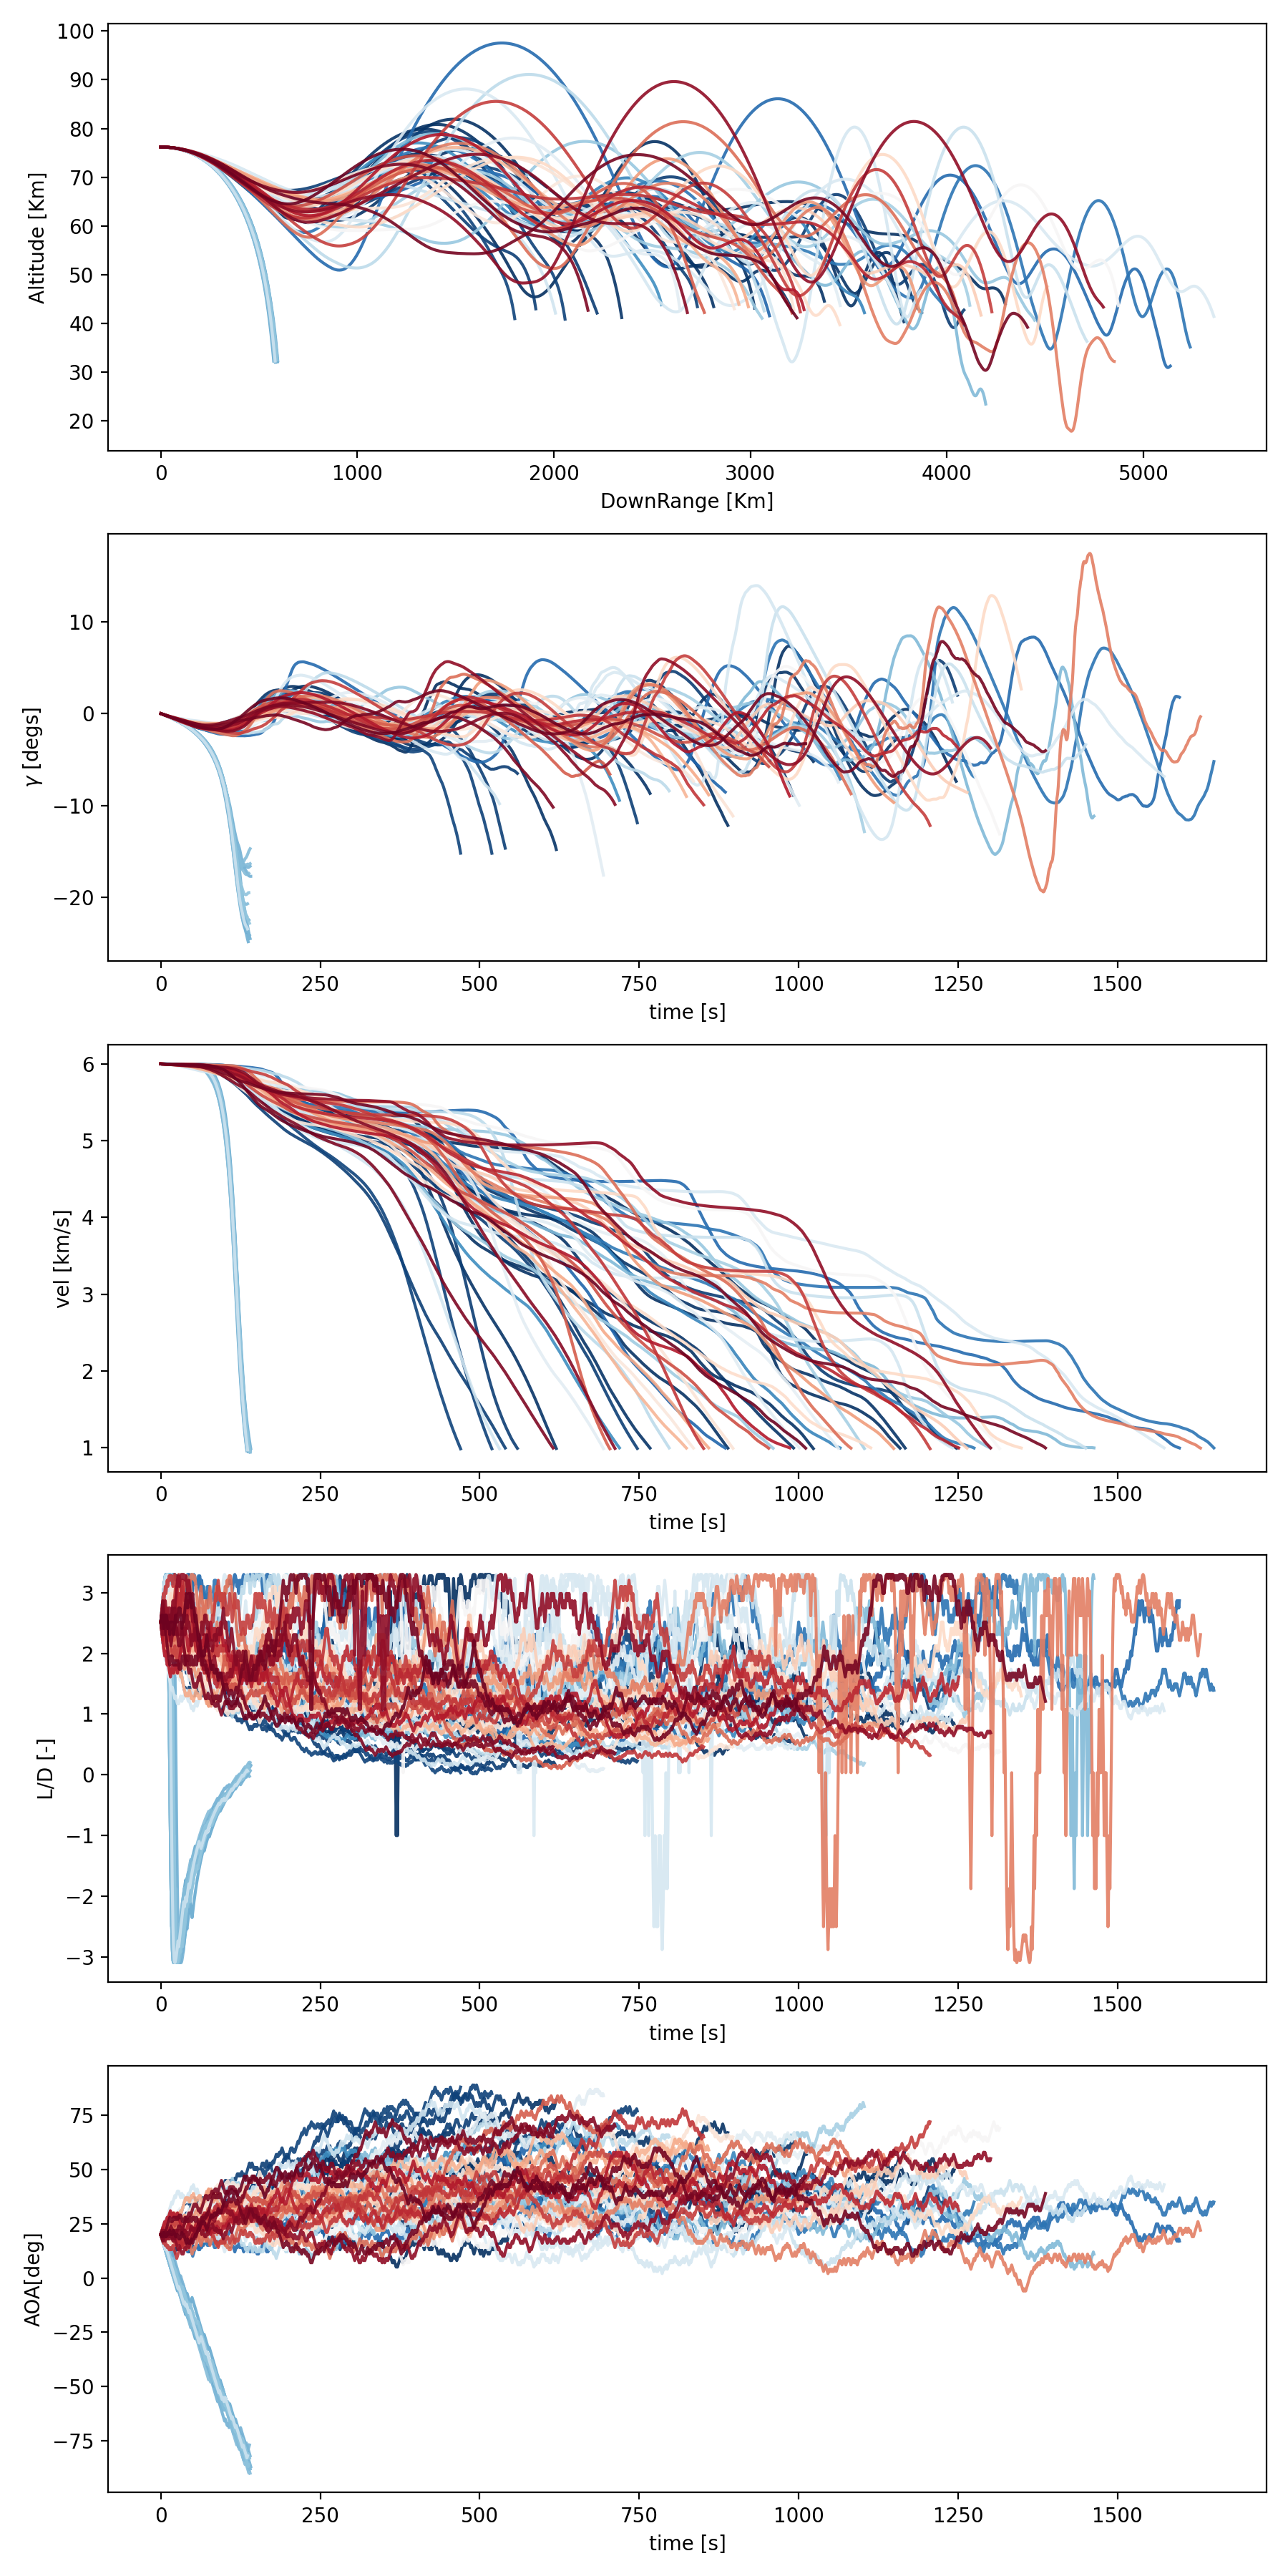
\includegraphics[width=\textwidth]{images/run_2.png}
     \caption{ Run 2}
     \label{fig:run_2}

   \end{subfigure}
   \begin{subfigure}[b]{0.5\textwidth}
     \centering
     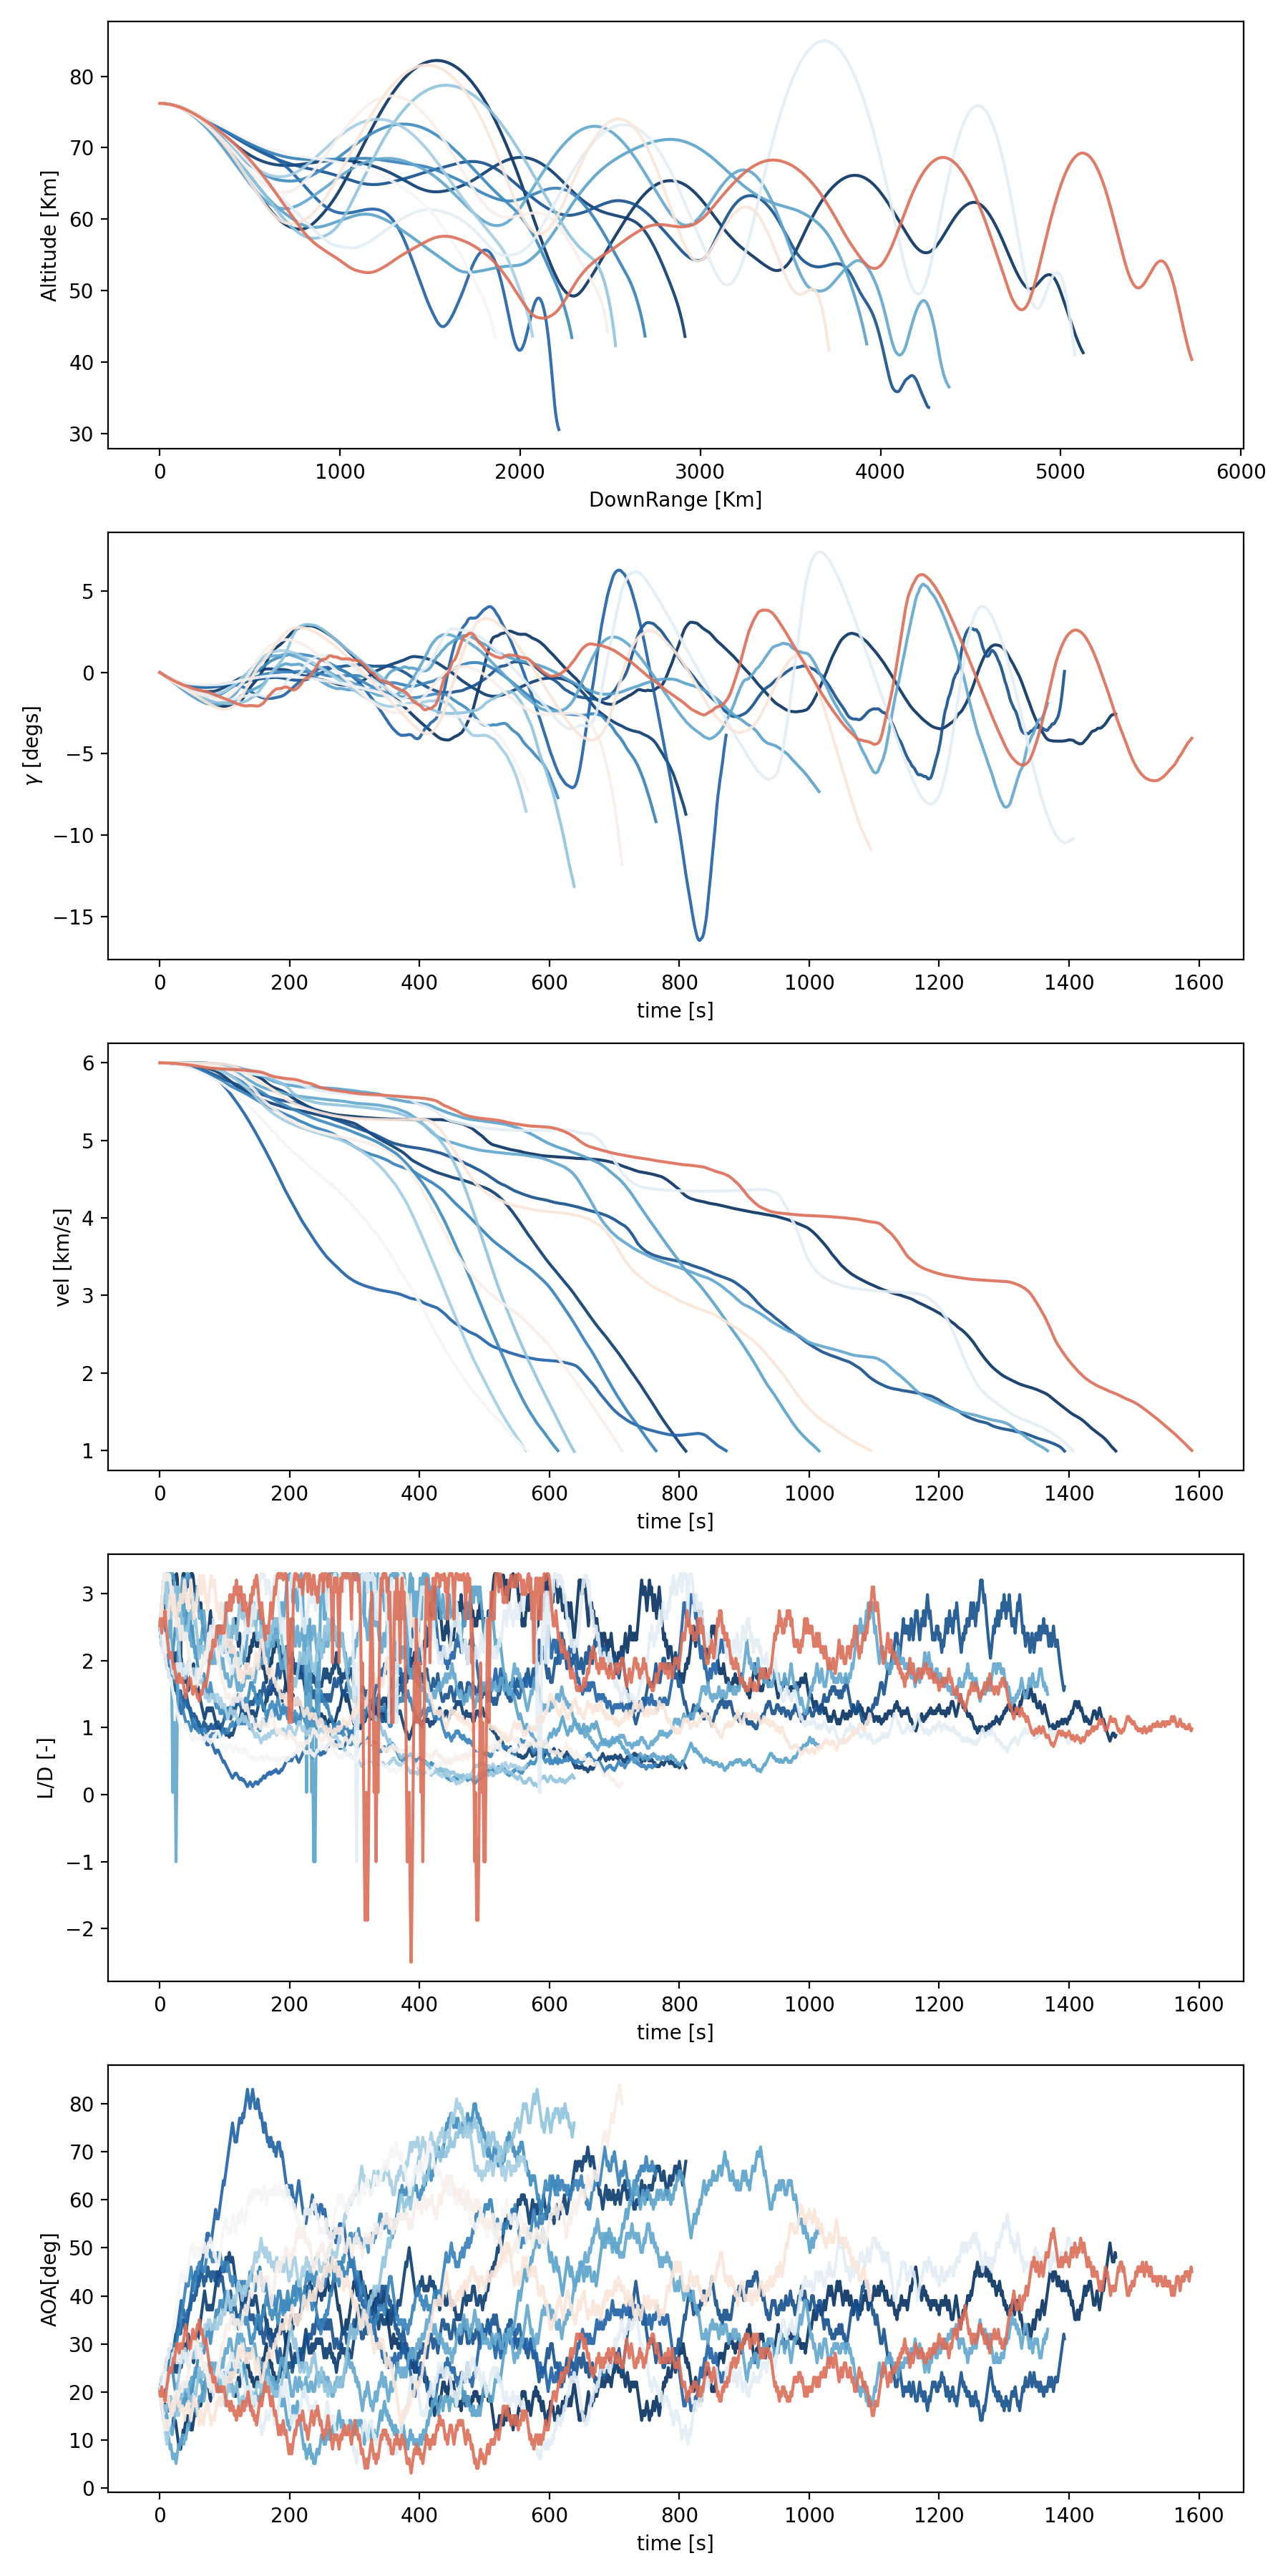
\includegraphics[width=\textwidth]{images/run_3.png}
     \caption{ Run 3}
     \label{fig:run_3}

   \end{subfigure}
   \caption{Output runs of DNN Q-learning. Blue signifies earlier portions of the training while red signifies later in training}
   \label{fig:training_data_plots}

\end{figure}
When we implement the policy after updating the results of two runs are shown in Figure \ref{fig:run_data_plots}. 
We see that the policy performance is acceptable for the earlier portions of the trajectory. However, as expected,
once velocities are lower more lift is needed to maintain level fligth. Hence, we see notable trends upward 
in subfigure \ref{fig:run_81}. We see in subfigure \ref{fig:run_82} just how sensitive initial chooses effect 
guidance for the policy. We note this by the subtle decrease in subfigure \ref{fig:run_81} as opposed to 
the increase in \ref{fig:run_82} leading to very different angle of attack progression but similar trajectory
profiles in altitudes.

\begin{figure}[H]
   \begin{subfigure}[b]{0.5\textwidth}
     \centering
     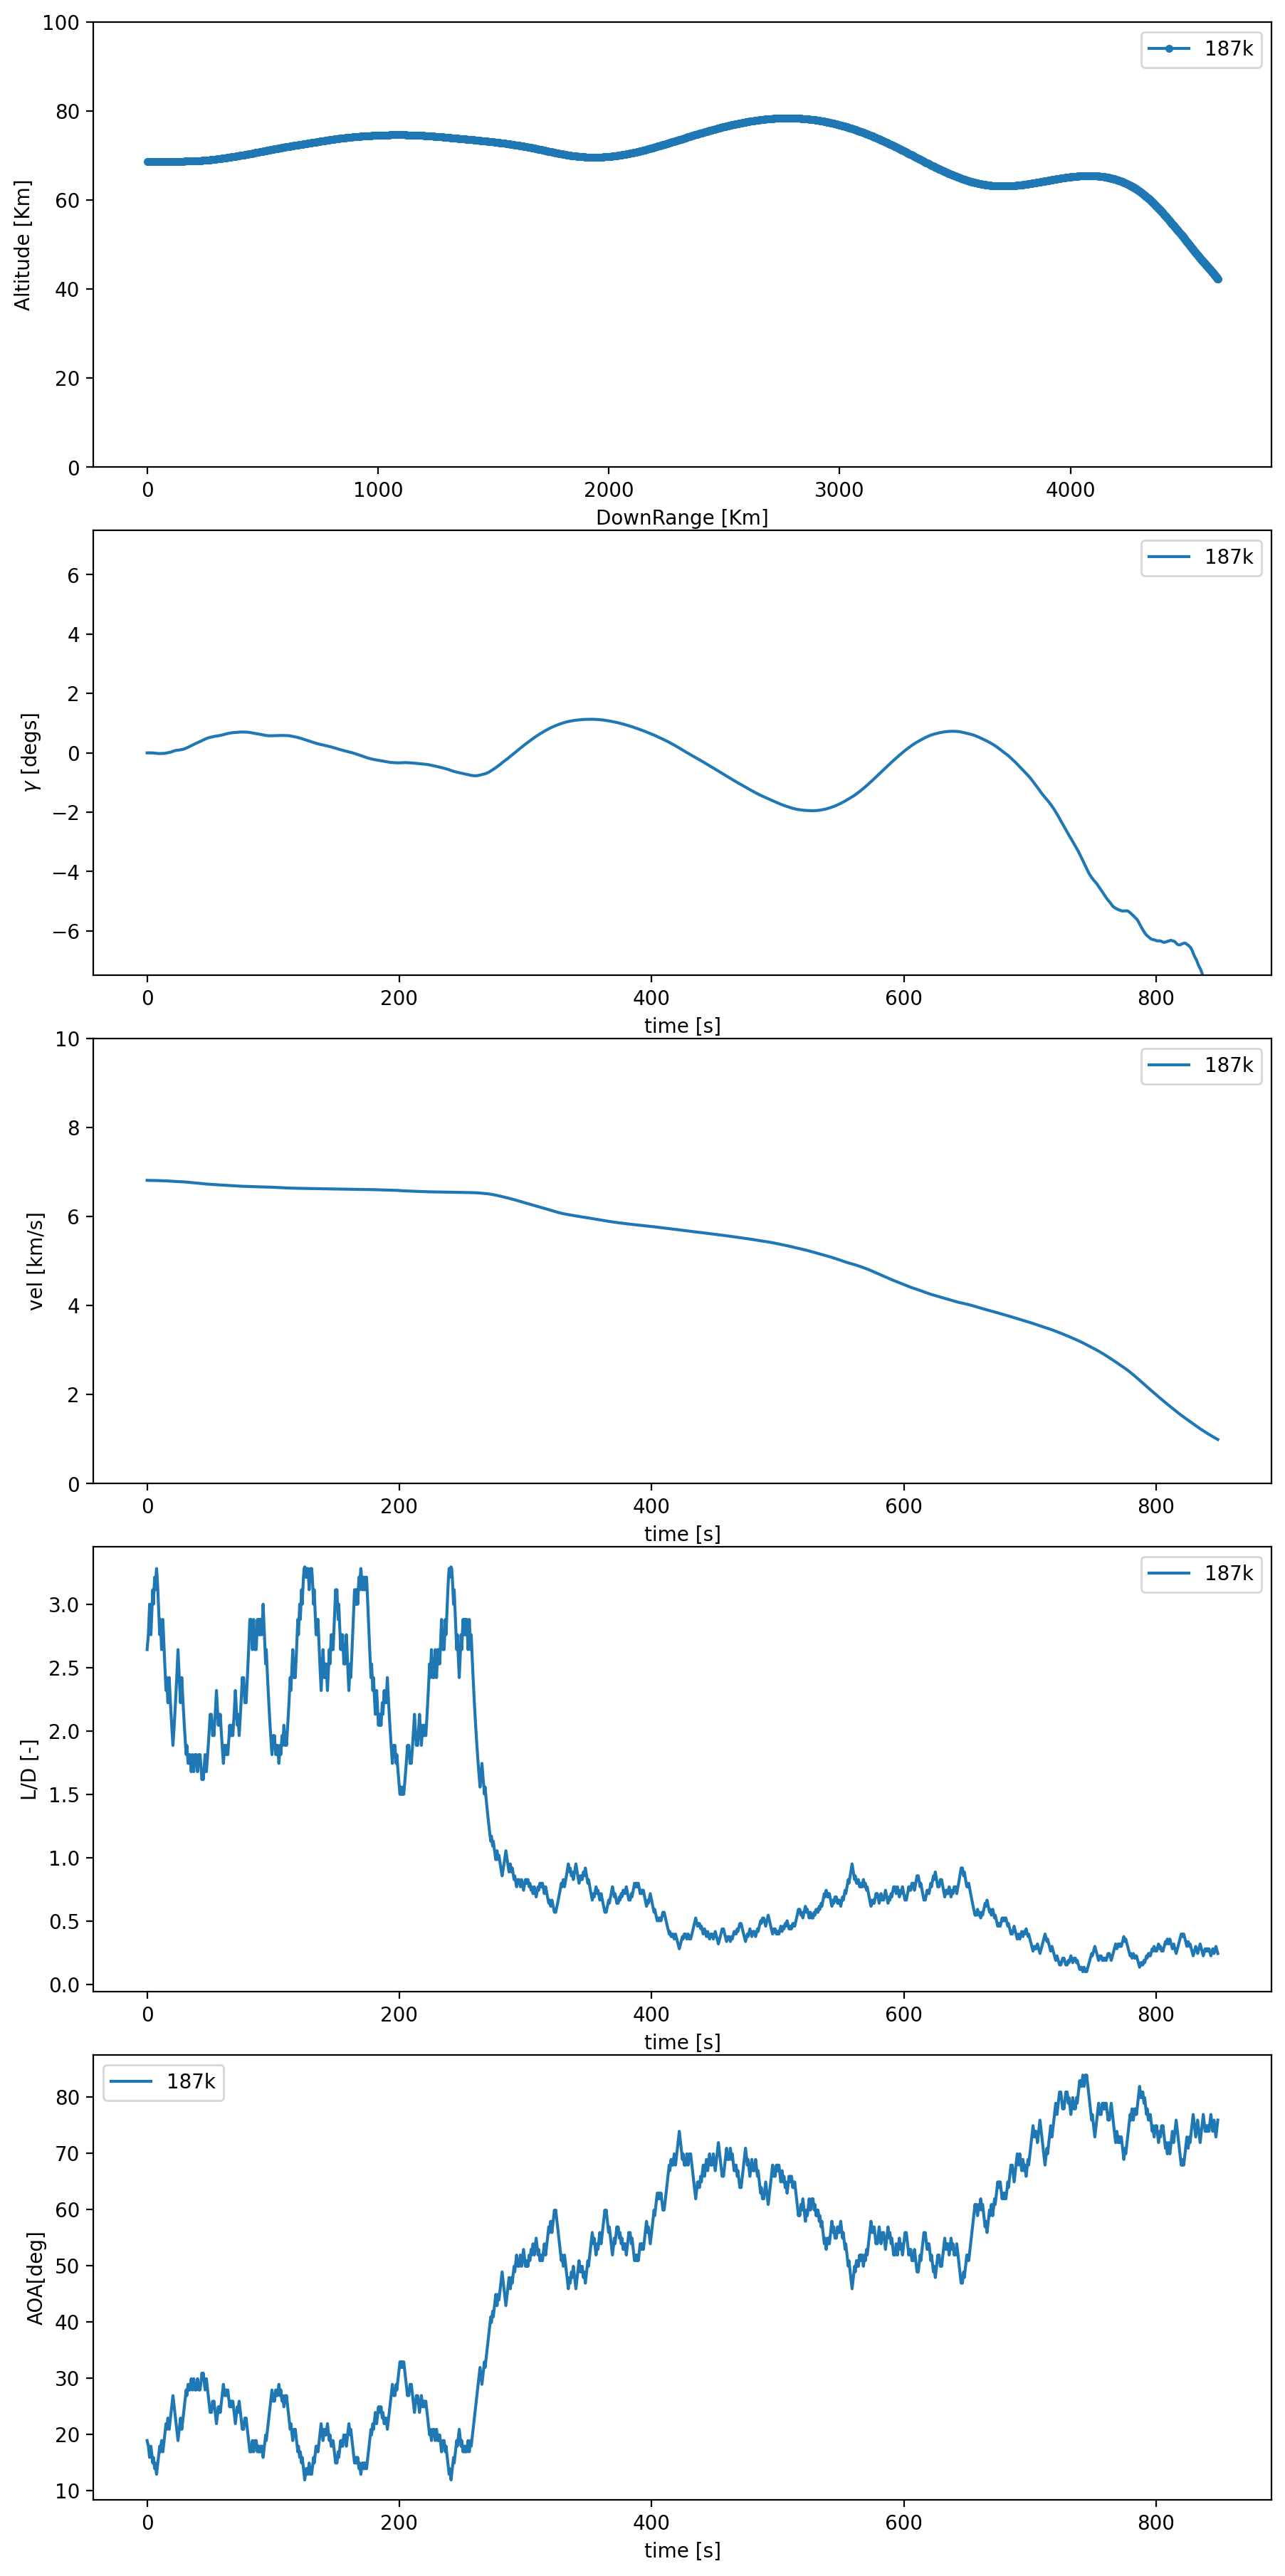
\includegraphics[width=\textwidth]{images/run8_explore.png}
     \caption{Testing optimal policy run 1}  
     \label{fig:run_81}
   \end{subfigure}
   \begin{subfigure}[b]{0.5\textwidth}
     \centering
     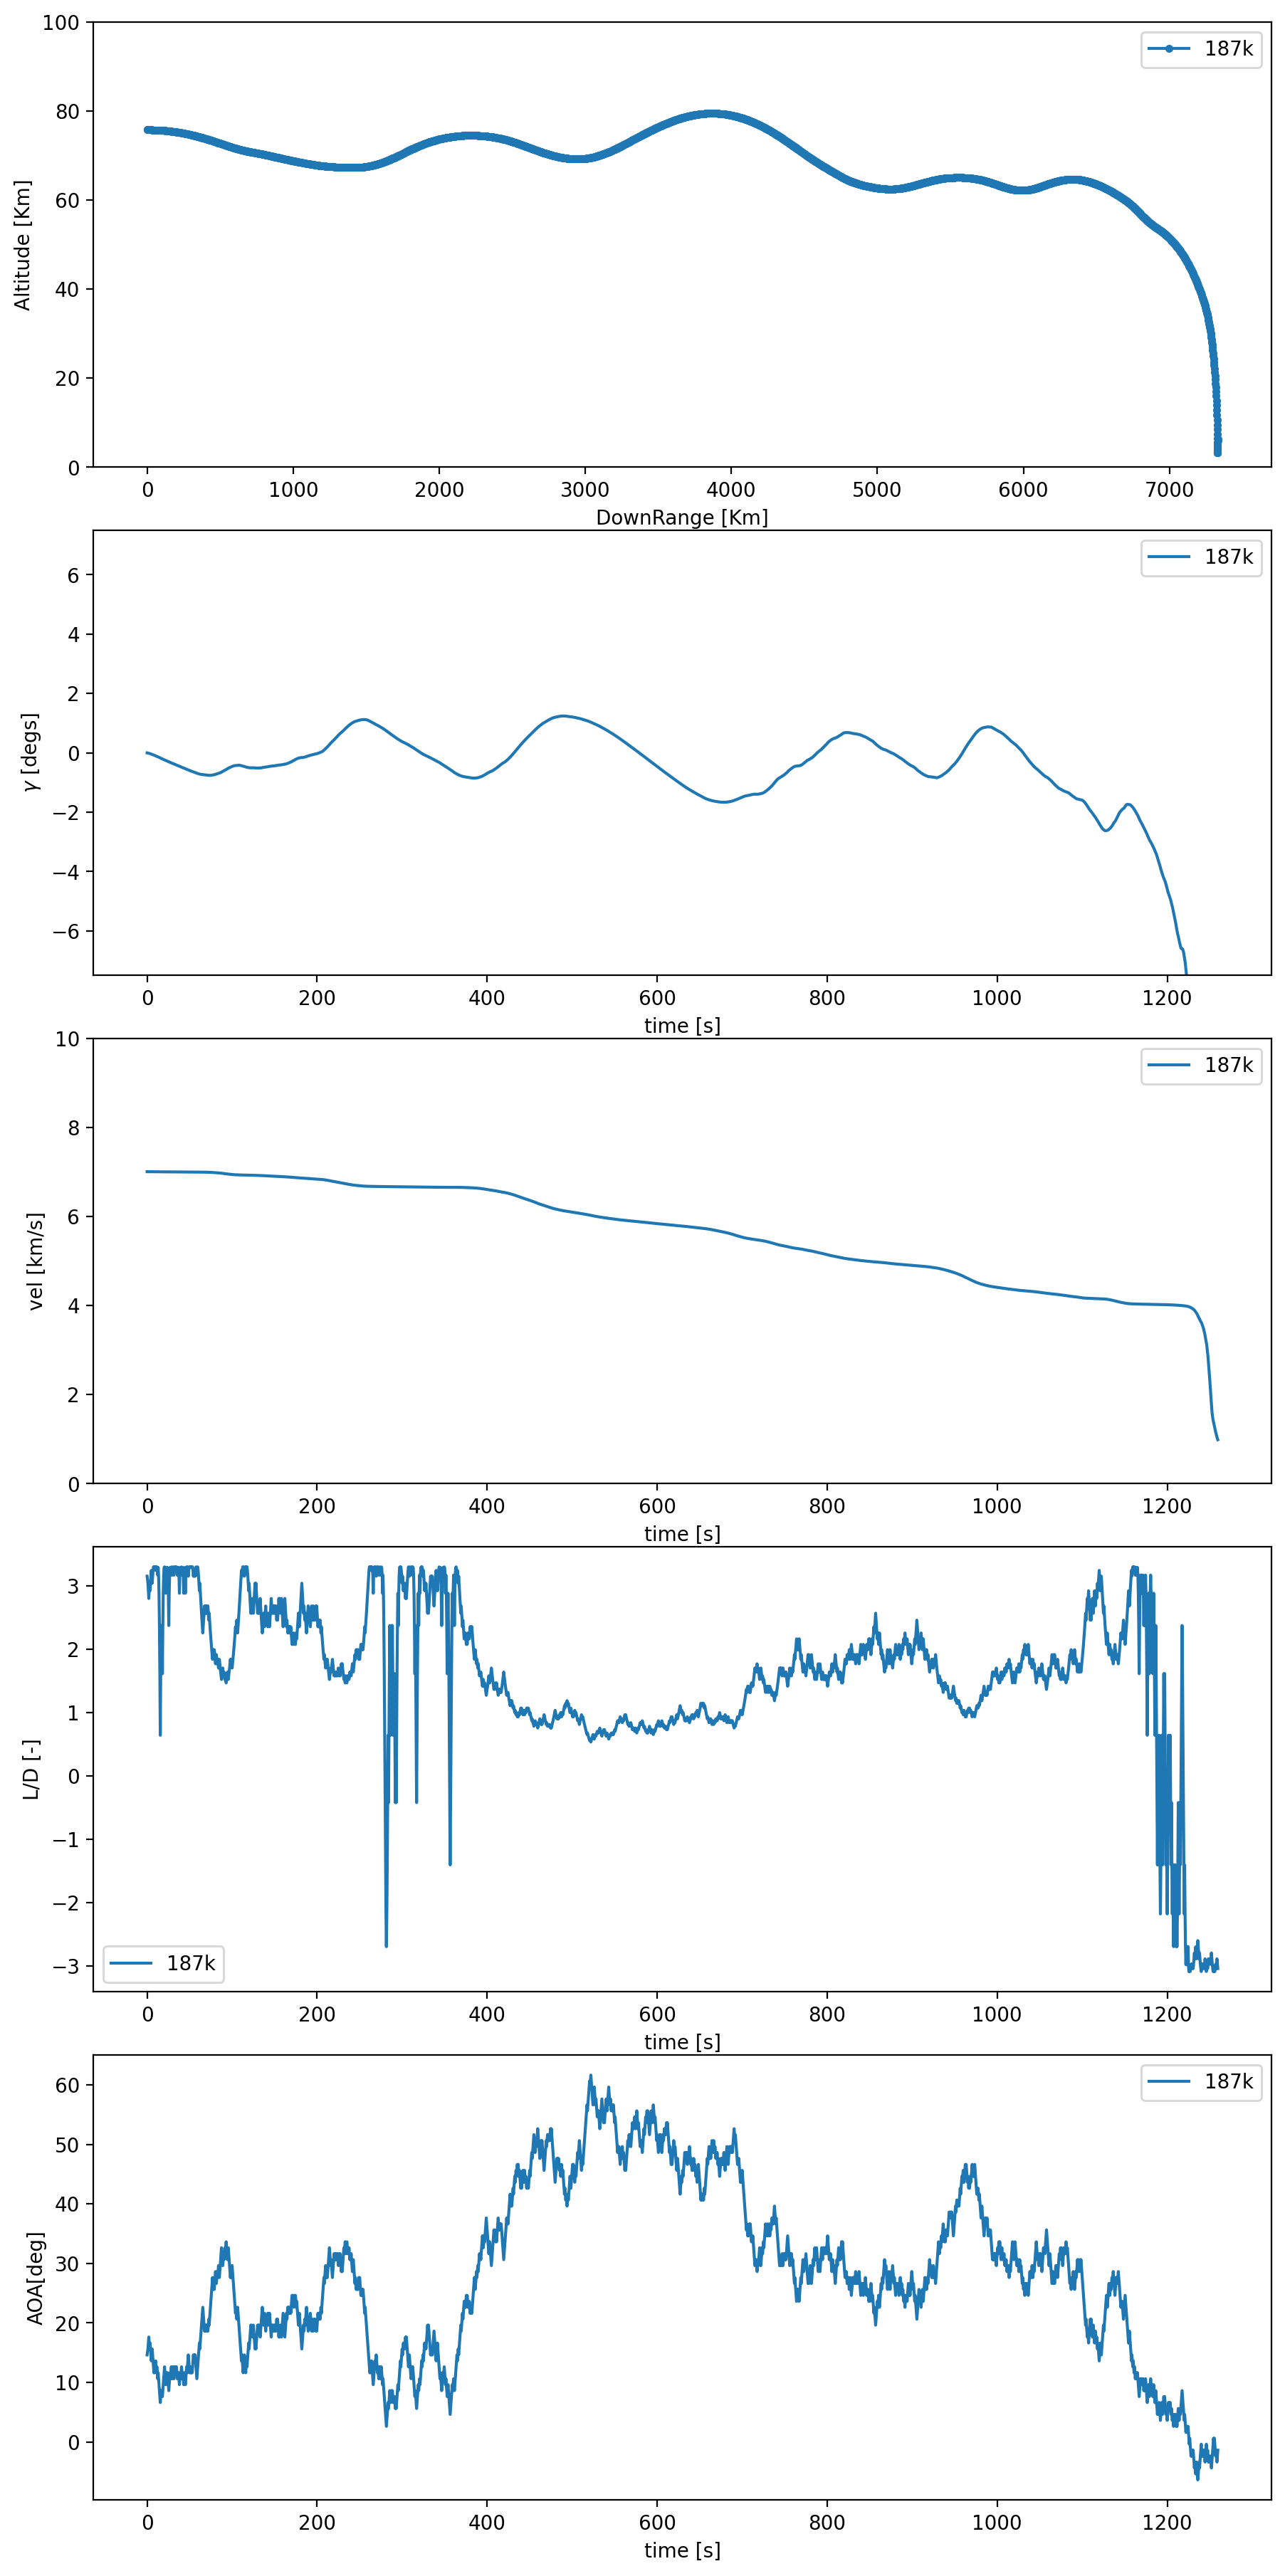
\includegraphics[width=\textwidth]{images/run8_explore2.png}
     \caption{ Testing optimal policy run 2}
     \label{fig:run_82}

   \end{subfigure}

   \caption{Online run of $\pi*$ after training}
   \label{fig:run_data_plots}

\end{figure}
\section{Discussion}
Compared with other MDP problems, this is more complex due to the usage of the ODE and there is no analytical solution 
for the controls problem. However, we have showed a new approach for simulating and controlling a hypersonic glide vehicle using simplified physics
and reinforment learning. Some of the key insights that we have discovered while doing this project is that firstly, Choosing a suitable neural network 
architecture for the policy and value functions was not trivial, as different architectures had different trade-offs in terms of complexity, 
performance, and generalization. We experimented with various architectures and compared their results to find the best one for our problem. Additionally, we have experienced that
uning the hyperparameters of the neural network and the reinforcement learning algorithm was also a difficult task, as they affected the convergence, stability, and robustness 
of the learning process. We used a trial-and-error approach and followed some best practices to find the optimal values for the hyperparameters.

We would report that our main issue was designing a proper reward function which was crucial for achieving our objective of maintaining a flat heading angle. 
We found that different reward functions had different impacts on the final output, and that some reward functions did not encourage the desired behavior. 
We also had to consider the trade-off between accuracy and computation time, as higher accuracy required more computation time and vice versa.

Some key limitations include the number of episodes that the model was trained on, even if it was then modeled to be generalizable for any initial condition. At the same time,
we also had difficulty in balancing multiple goals, such as minimizing the heading angle but also not having it to terminate too early. Afterwards, due to the scope of the simplified physics
it terminates early after the altitude reaches a high height. Qualitatively, this trajectory is good because there was not that much reduction in velocity while also having a straight heading angle.
Unfortunately, this better controls can't be used or it won't be physically intuitive. In the end, we had to settle but something mediocre but was still able to perform better than the constant angle-of-attack.

\section{Conclusions}
In conclusion, we have showed the feasibility of using a neural net for reinforcement 
learning of a hypersonic glide vehicle. This was achieved by running multiple episodes and was split into an exploration, 
training, and testing state. In the exploration stage, the action taken was completely random, while in the training stage, 
the randomness of the action choosing was slowly decreasing. With our goal of having a flat heading angle, the new trajectory 
of the HGV is much different than the constant angle of attack case. There were lots of issues that was faced during the 
simulation for each run because of the limitations on some of the state space values so it is still physically representative 
and accurate. Overall, in addition with training hyperparameters, this was addressed by changing the rewards, termination 
and neural net hyperparameters. And was able to get a proper control system using the first few timesteps of the gliding. 

For future work, extended training time and a more complex neural network architecture may train the controller better 
to fit our objectives more accurately. A neural network generally gets more complex with various combinations of sequential 
blocks and activation functions as the model to be trained gets more complicated. In this case, with a 3 layer fully connected layer, 
this is definitely not enough as the number of nodes cannot fully represent a complex 4 state ordinary differential equation. Different work
in the realm of machine learning has been done with the use of LSTMs or Residual Blocks which add complexity. Additionally, it can be noted that
neural networks have a tendency to overfit the data so the use of dropout layers may benefit the model.

\newpage
\section*{Appendix}
\subsection*{ Trajectories with constant angle-of-attack }
\begin{figure}[hbt!]
    \begin{subfigure}[b]{0.5\textwidth}
      \centering
      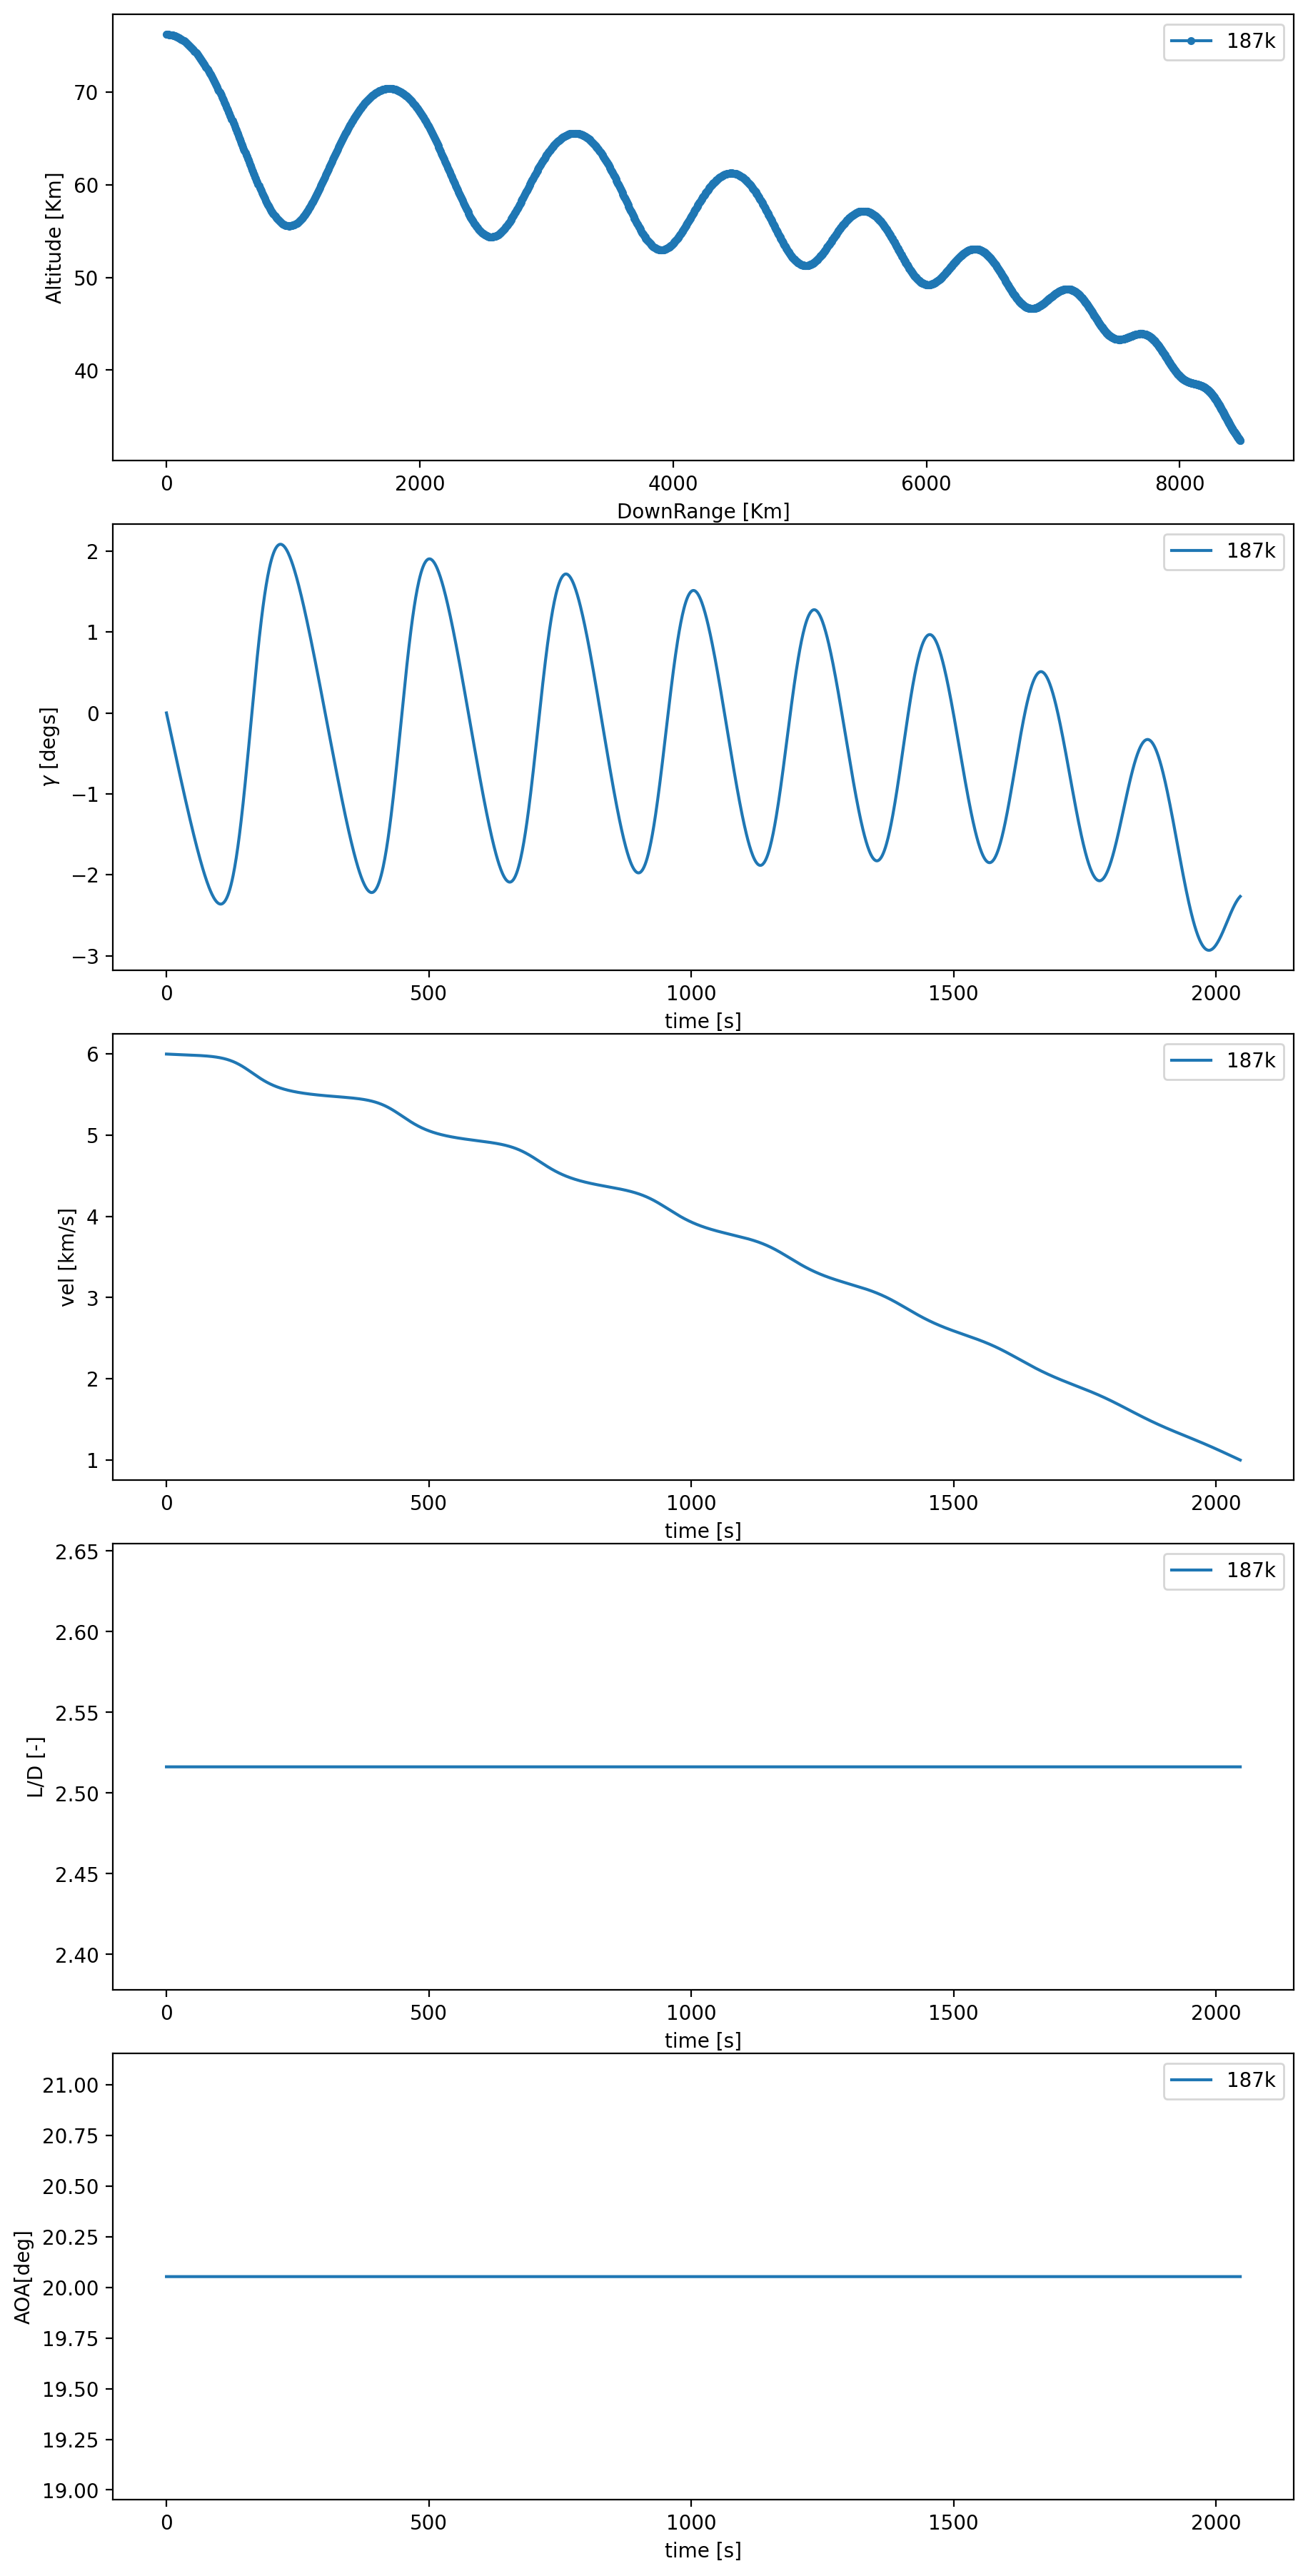
\includegraphics[width=\textwidth]{images/og1.png}
      \caption{ vel = 6km/s,  alt=76.2 km,   $\alpha$=20.05}
    \end{subfigure}
    \begin{subfigure}[b]{0.5\textwidth}
      \centering
      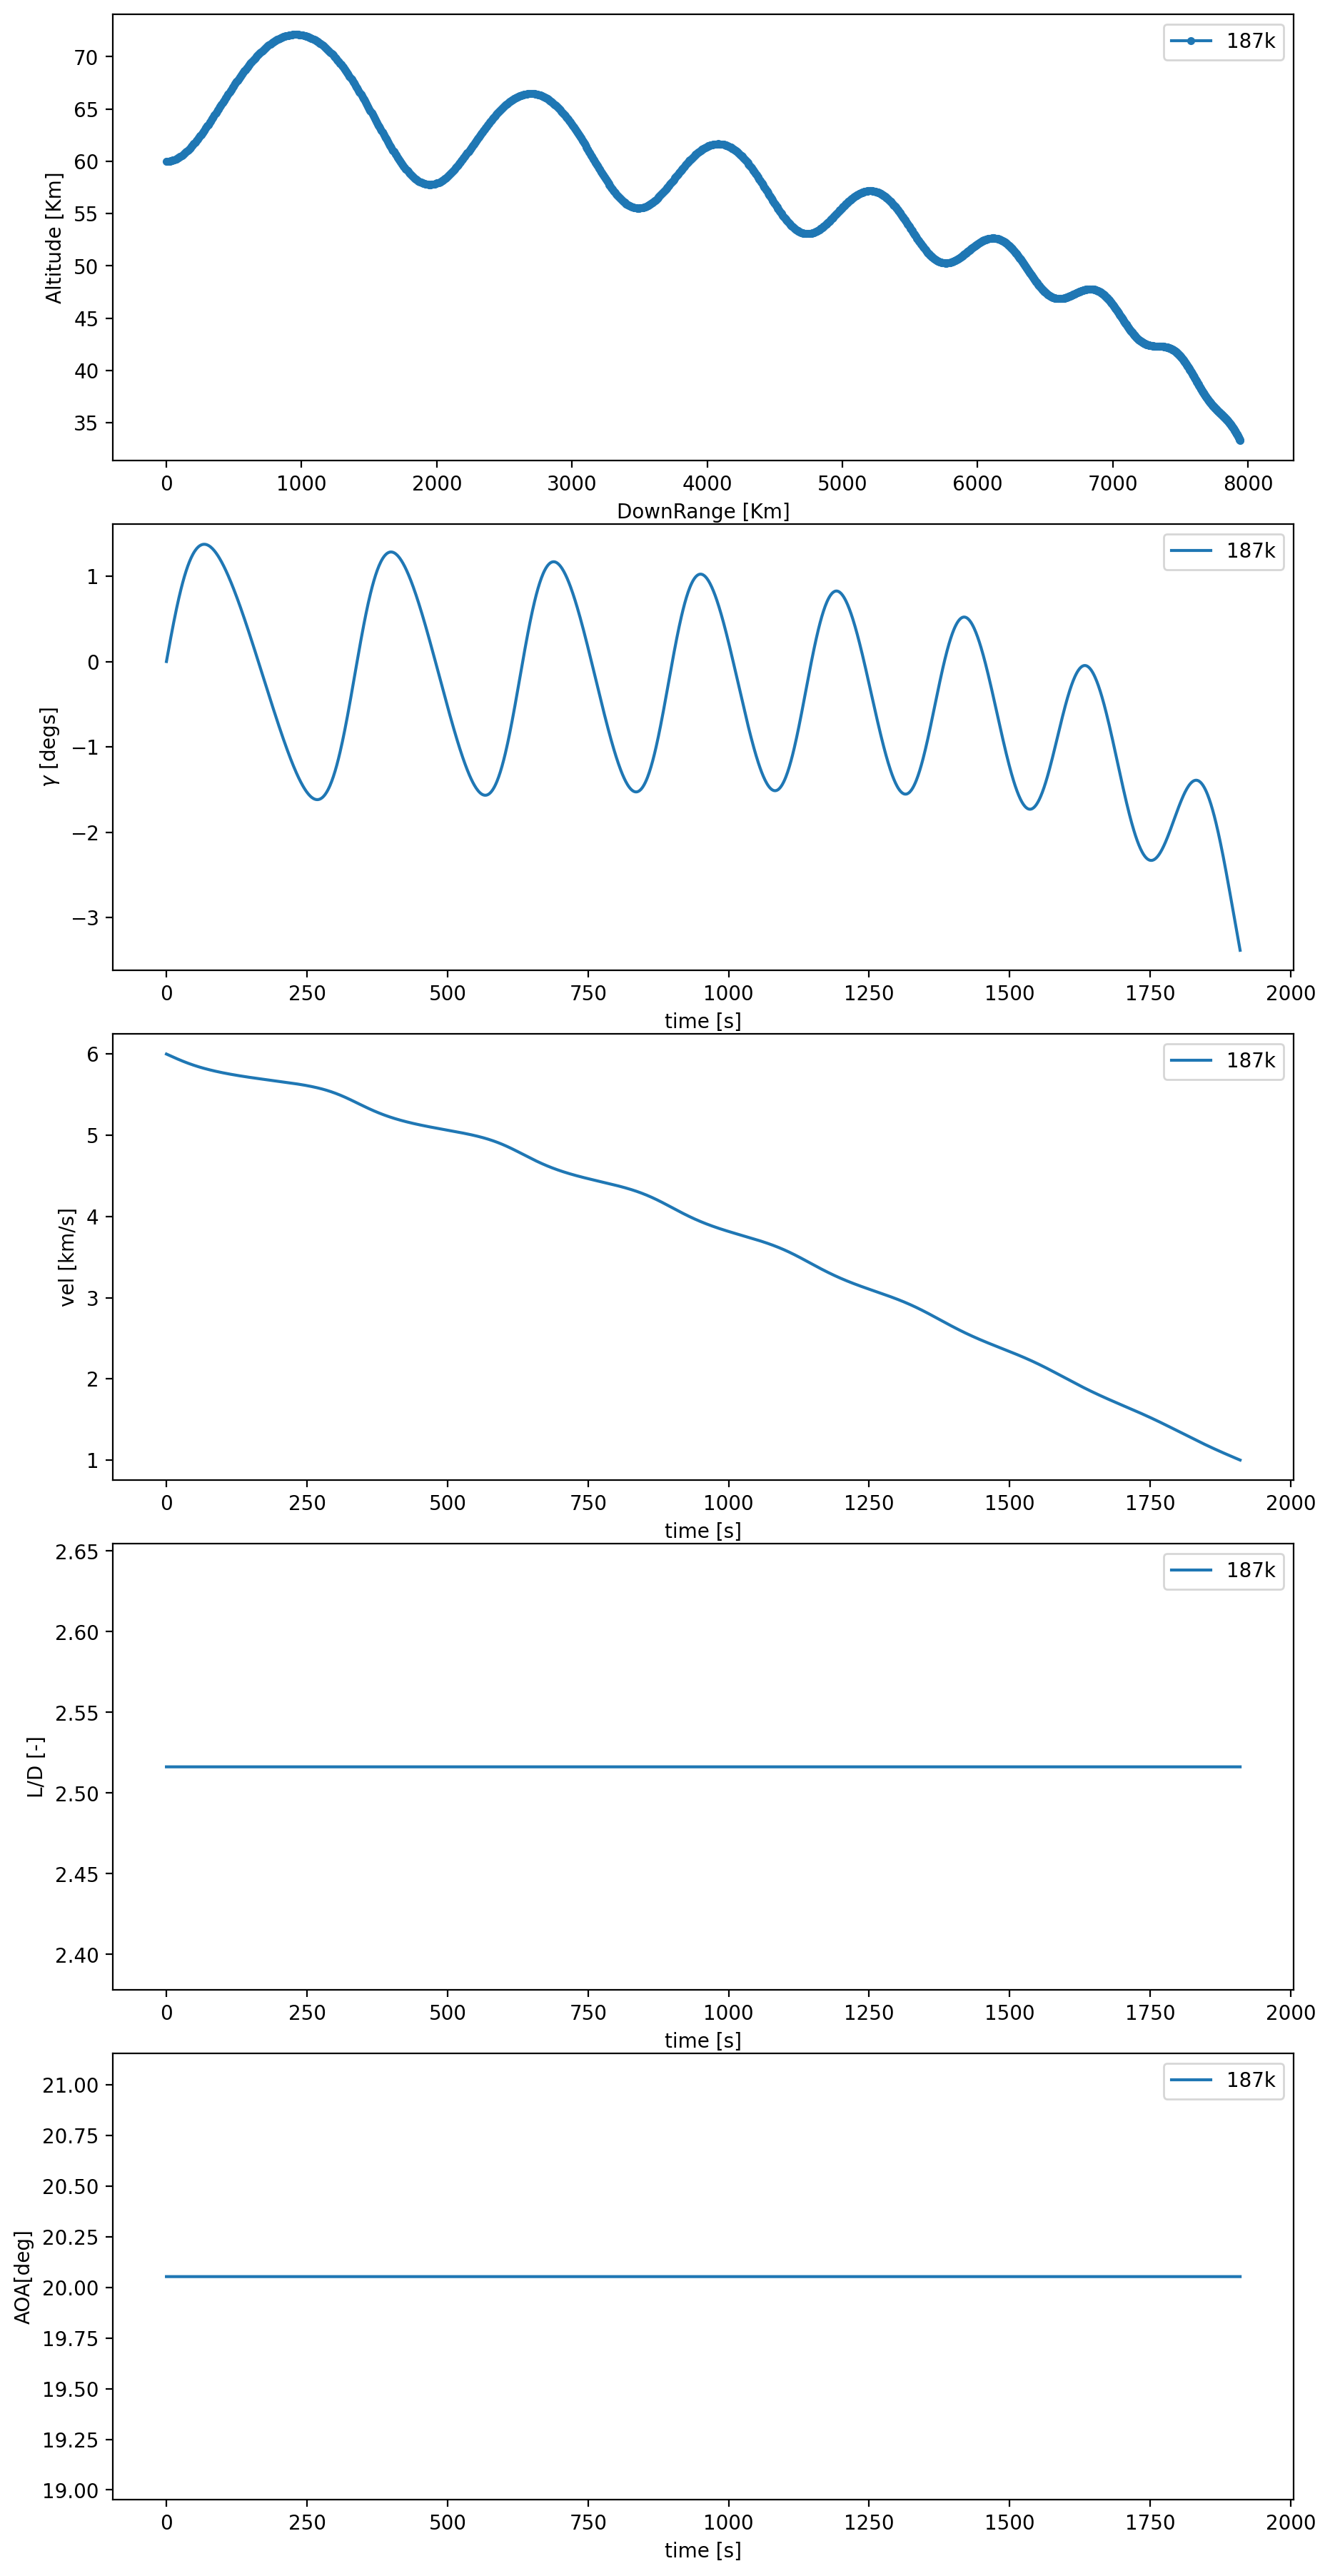
\includegraphics[width=\textwidth]{images/og2.png}
      \caption{ vel = 6km/s,  alt=60.0 km,   $\alpha$=20.05}
    \end{subfigure}
\end{figure}

\newpage
\subsection*{ Hypersonic Glide Vehicle Environment }
\lstset{style=mystyle}
\lstinputlisting[language=Python]{code/sim_NeuralNet.py}

\newpage
\subsection*{ Neural Network with Deep Q-Learning }
\lstset{style=mystyle}
\lstinputlisting[language=Python]{code/NeuralNet_jj.py}

\end{document}
\documentclass[11pt]{article} % For LaTeX2e
\usepackage{rldmsubmit,palatino}
\usepackage{graphicx}
\usepackage{verbatim} 
\usepackage{amsmath} % for 'bmatrix' environment
\usepackage{subcaption} % sub-figures with sub-labels
\usepackage{algpseudocode}

%%% Code Listing 
\usepackage{listings}
\usepackage{xcolor}

\definecolor{codegreen}{rgb}{0,0.6,0}
\definecolor{codegray}{rgb}{0.5,0.5,0.5}
\definecolor{codepurple}{rgb}{0.58,0,0.82}
\definecolor{backcolour}{rgb}{0.95,0.95,0.92}
\usepackage{listings}
\usepackage{tcolorbox}
\tcbuselibrary{listings}

\lstdefinestyle{mystyle}{
	backgroundcolor=\color{backcolour},   
	commentstyle=\color{codegreen},
	keywordstyle=\color{magenta},
	numberstyle=\tiny\color{codegray},
	stringstyle=\color{codepurple},
	basicstyle=\ttfamily\footnotesize,
	breakatwhitespace=false,         
	breaklines=true,                 
	captionpos=b,                    
	keepspaces=true,                 
	numbers=left,                    
	numbersep=5pt,                  
	showspaces=false,                
	showstringspaces=false,
	showtabs=false,                  
	tabsize=2
}
% sub-figures with sub-labels
\usepackage{subcaption}
\usepackage{float}
\usepackage[]{placeins}
\begin{comment}
   Applied Project: In the final report you should introduce the problem you solved 
   and the techniques used to solve the problem. If multiple algorithms were used 
   compare the performance of the different algorithms. If possible show how the 
   algorithms perform (accuracy and computation time) as the size of the problem 
   increases. If relevant show how your solutions methods perform if the model is 
   not accurately specified. Discuss any insights you have gained about your problem 
   as well as any insights about the best solution algorithm. Include a discussion 
   of potential shortcomings of your solution or problem formulation and how you 
   can improve these things. In addition, discuss possible extensions of your work.
\end{comment}
   

\title{Application of RL to Simulate Performance of an Unguided Hypersonic Glide Vehicle}


\author{
Justine John A Serdoncillo \\
Aerospace Engineering and Mechanics\\
University of Minnesota - Twin Cities\\
Minneapolis, MN  55414\\
\texttt{serdo004@umn.edu} \\
\And
Darryl Williams \\
Aerospace Engineering and Mechanics\\
University of Minnesota - Twin Cities\\
Minneapolis, MN  55414\\
\texttt{will7322@umn.edu} \\
}

% The \author macro works with any number of authors. There are two commands
% used to separate the names and addresses of multiple authors: \And and \AND.
%
% Using \And between authors leaves it to \LaTeX{} to determine where to break
% the lines. Using \AND forces a linebreak at that point. So, if \LaTeX{}
% puts 3 of 4 authors names on the first line, and the last on the second
% line, try using \AND instead of \And before the third author name.

\newcommand{\fix}{\marginpar{FIX}}
\newcommand{\new}{\marginpar{NEW}}

\begin{document}

\maketitle

\begin{comment}
\begin{abstract}

The \emph{title} should be a maximum of 100 characters. 

The \emph{abstract} should be a maximum of 2000 characters of text,
including spaces (no figure is allowed). You will be asked to copy
this into a text-only box; and it will appear as such in the
conference booklet. Use 11~point type, with a vertical spacing of
12~points.  The word \textbf{Abstract} must be centered, bold, and in
point size 12. Two line spaces precede the abstract.
Our project aims to simulate the performance of a high-speed aircraft using simplified physics.
We have chosen an unguided hypersonic glide vehicle (HGV) as the exemplar case. The primary
objective is to develop a control policy that ensures the vehicle maintains a straight heading. Typ-
ically, achieving this would involve approximating derivatives or deriving analytical expressions
for application in a feedback controller.
However, we are taking a different approach by utilizing reinforcement learning (RL) to create
an optimal policy for maintaining the heading angle.
\end{abstract}

\keywords{
Q-Learning, Neural Networks, Glide Vehicles
}

\acknowledgements{We are deeply indebted to Google DeepMind and
the Weinberg Institute for Cognitive Science for
their generous support of RLDM2017.}  

\startmain % to start the main 1-4 pages of the submission.
\section{Submission of papers to RLDM}

RLDM requires electronic submissions.  This year's electronic
submission site is   
\begin{center}
   https://cmt3.research.microsoft.com/RLDM2017/
\end{center}

Please read the instructions below, and follow them faithfully. Note
that there is also a template \verb+rldm.rtf+ for Microsoft Word,
which is available from the website below.
\subsection{Style}

Papers to be submitted to RLDM must be prepared according to the
instructions presented here. Papers consist of a \emph{title}, which
has a maximum of 100 characters, an \emph{abstract}, which is a
maximum of 2000 characters, up to five key words, and an
\emph{extended abstract}, which starts on the second page, and can be
between one and four pages. Figures and references should be included
in the latter.

Authors preferring \LaTeX{} are requested to use the RLDM \LaTeX{}
style files obtainable at the RLDM website at
\begin{center}
   http://www.rldm.org/
\end{center}
The file \verb+rldm.pdf+ contains these instructions and illustrates
the various formatting requirements your RLDM paper must
satisfy. There is a \LaTeX{} style file called \verb+rldmsubmit.sty+,
and a \LaTeX{} file \verb+rldm.tex+, which may be used as a ``shell''
for writing your paper. All you have to do is replace the author,
title, abstract, keywords, acknowledgements and text of the paper with
your own. The file
\verb+rldm.rtf+ is provided as an equivalent shell for Microsoft Word users. 

\section{General formatting instructions}
\label{gen_inst}

The paper size for RLDM is ``US Letter'' (rather than ``A4''). Margins
are 1.5cm around all sides. Use 11~point type with a vertical spacing
of 12~points. Palatino is the preferred typeface throughout.
Paragraphs are separated by 1/2~line space, with no indentation.

Paper title is 17~point, initial caps/lower case, bold, centered between
2~horizontal rules. Top rule is 4~points thick and bottom rule is 1~point
thick. Allow 0.6cm space above and below title to rules. 

The lead author's name is to be listed first (left-most), and
the co-authors' names (if different address) are set to follow. If
there is only one co-author, list both author and co-author side by side.

\section{Preparing PostScript or PDF files}

Please prepare PostScript or PDF files with paper size ``US Letter''.
The -t letter option on dvips will produce US Letter files.
\end{comment}

\begin{abstract}. 
   
   In this paper, we present a novel approach for simulating and controlling a 
   high-speed aircraft using simplified physics and reinforcement learning (RL).
   We focus on the case of an unguided hypersonic glide vehicle (HGV), 
   which is a challenging and relevant problem for aerospace engineering.
   Our goal is to design a control policy that can keep the vehicle on a straight heading, 
   without relying on analytical expressions or numerical approximations of the dynamics. 
   To achieve this, we use neural networks to model the continuous state space 
   and the action space of the system, and apply RL algorithms to learn the optimal policy from data. 
   We compare our approach with conventional methods and demonstrate its effectiveness 
   and robustness in various scenarios. Our results show that RL can offer a 
   viable and efficient alternative for controlling high-speed aircraft.
\end{abstract}
   
\keywords{Q-Learning, Neural Networks, Glide Vehicles}

\section{Problem Introduction}
Hypersonic glide vehicles (HGVs) are capable of maneuvering within earth's atmosphere as they glide at high-speeds
in excess of Mach 5. As a result of their speed, HGVs are able to travel several thousand kilometers within a short
amount of time. Their ability to achieve long distances in short time frames and their use of aerodynamic forces for
maneuvering have made them a subject of extensive research, particularly for defense applications.
A typical trajectory for HGVs involves a boost phase that brings the vehicle high in the atmosphere, a reentry phase,
and a glide phase at speeds of Mach 5-20. 

In this paper we use a deep Q-learning approach with experience reply to perform guidance on an HGV during its glide 
phase. In the implemented framework, an aerodynamic code is integrated into the equation of motion over a 
non-rotating spherical Earth:

\begin{equation}
   \frac{\partial}{\partial t}
   \begin{bmatrix}
       \gamma \\
       V \\
       x \\
       h 
   \end{bmatrix} =
   \begin{bmatrix}
       \frac{1}{V} \left[\frac{L}{m}+g \cos(\gamma)-\frac{V^2}{R} \cos(\gamma)\right] \\
       \frac{D}{m}+ g\sin(\gamma)\\
       -V\cos(\gamma) \\
       -V\sin(\gamma)
   \end{bmatrix} \, .
   \label{eqn:EOM}
\end{equation}

We then use an optimal policy $\pi^*$, to preform guidance on the HGV initial conditions of 60 km in altitude traveling
at 6 km/s. Newtonian Aerodynamic (NA) was used as a lower-fidelity tool to compute the aerodynamic forces acting on the
HGV. This approximate method is much cheaper than computational fluid dynamics enabling rapid exploration of the simulated
environment but for lower levels of accuracy. Newtonian aerodynamics assumes tangential velocities are unchanged, while the
normal velocity results in aerodynamic forces acting on the vehicle as shown in figure \ref{fig:NA}. 
\begin{figure}[H]
   \centering
     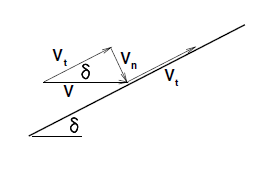
\includegraphics[width=0.5\textwidth]{images/NA.png}
   \caption{Illustration of tangential and normal velocities on surface.}
   \label{fig:NA}
\end{figure}
This approximation is more accurate as speeds are increased into higher mach numbers. The algorithm to compute forces over
a tessellated surface is described in the NA Procedure below.

\begin{algorithmic}
   \State $N =$ number of triangles elements
   \Procedure{NA}{$\alpha$} %\Comment{The g.c.d. of a and b}
       \State $i \gets 1$
   \State $\hat{v} =\{\cos(\alpha),sin(\alpha),0\} $
   \State Forces =$\{0,0,0\} $
   \While{$i \leq N$}
   \If{$(\hat{v} \cdot \hat{n}_i) < 0$}
       \State  ${cp}_i = 2 \left(\hat{v} \cdot \hat{n}_i\right)^2$
   \Else
       \State  ${cp}_i = 0$ \Comment{Flow is hidden from velocity vector}
   \EndIf
   \State  $P_i=({cp}_i \cdot q)+P_{\infty}$
   \State  $F = F + (P_i \cdot A_i)\cdot(-\hat{n}_i) $\Comment{$A_i$  computed from cross product}
   \State $i \gets i+1$
   \EndWhile
   \State  $D=F(2)\sin(\alpha)+F(1)\cos(\alpha)$
   \State  $L=F(2)\cos(\alpha)-F(1)\sin(\alpha)$
   \EndProcedure
\end{algorithmic}

We then use the aerodynamic forces(L,D) to compute the derivatives in Equation \ref{eqn:EOM}. Time was integrated using the
4-th order Runga-Kutta method with a fixed time-step of $\Delta t = 1$ seconds as the time discretization. 

\section{Methodology}
   \subsection{Simulation Environment}
   Our policy $\pi$(a = $\alpha|s$), when given a state, selects an angle of attack ($\alpha$) such that forces on the
   vehicle, lift ($L$) and drag ($D$), are modulated. With these forces, we can then integrate the equation of motion
   for a fixed $\delta t$ to arrive at out new state. We note that the simulated environment is not representative
   of actual flight. Rather, this model for system dynamics is sought as a proof of concept and to have tractable 
   training times of the algorithm used. The relative disparity between system dynamics comparing a computational  
   fluid dynamics approach to NA is shown in Figure \ref{fig:compare}.
   \begin{figure}[H]
      \centering
        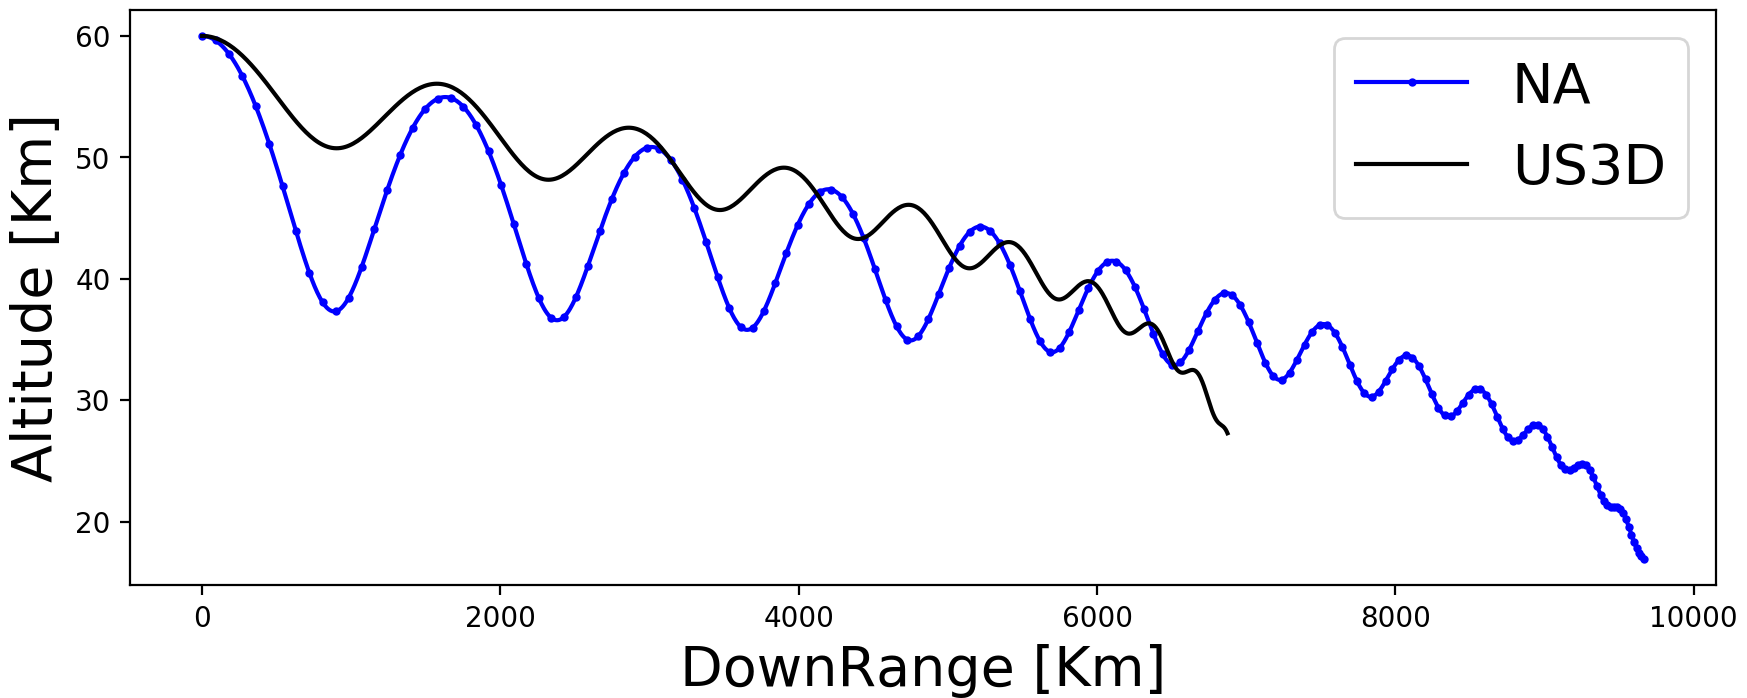
\includegraphics[width=0.65\textwidth]{images/compare_alt.png}
        \caption{Comparison between full trajectory using US3D (CFD) and NA. }
        \label{fig:compare}

   \end{figure}
\subsection{Markov Decision Process model}
We implemented an epsilon greedy approach for exploration. Modeled as an episodic problem that terminated once the
altitude went below 1 km or velocity decreased below 1 km/s. A summary of major hyperparameters and state space below:
\begin{itemize}
   \item State Space: $\gamma$, $h$,$V$
   \item Action: $\alpha$
   \item $\epsilon_{i+1} = 1+ \log(\epsilon_i/(0.6*n))$
   \item  Problem: Episodic with gamma = 0.9 
   \item Rewards: $- \gamma^2$ + d
\end{itemize}


\subsection{Neural Networks for continuous State Space RL}
Artificial neural networks have been used for extensively for nonlinear function approximation. 
It characterized by applying a linear model to a feature vector then applying a non-linear mapping.
This neural networks are often convoluted within each other its to have several instances of linear and non-linear 
mappings applied to them. This type of neural network architecture is known as a deep neural network. For the 
implemented method we decided on a neural network composed of two 24 neuron hidden layers, The non-linear activation
decided was the use of the rectified linear unit. 

In our case, we are using a deep Q-learning methodology by using an input tuple of the state, action, new state, and the reward. Our 
compute time was broken into the following:
\begin{itemize}

   \item Exploration: first 25\%
   \begin{itemize}
      \item choosing random actions to explore the state transitions
      \item store [state, action, state prime, reward] for each combination
   \end{itemize}
   
   \item Training: second 65\%
   \begin{itemize}
      \item reduction of epsilon to reduce exploration
      \item trains using stored memory
      \item input is the state and action, output is the next state and reward
   \end{itemize}
   
   \item Testing: last 10\%
   \begin{itemize}
      \item test neural net by running on new intial conditions and trajectories
   \end{itemize}
   
   \end{itemize}
   
   The figure below shows the algorithm that we based our neural network on. The code for the environment and neural network as seen in the appendices below.
   
   \begin{figure}[H]
      \centering
        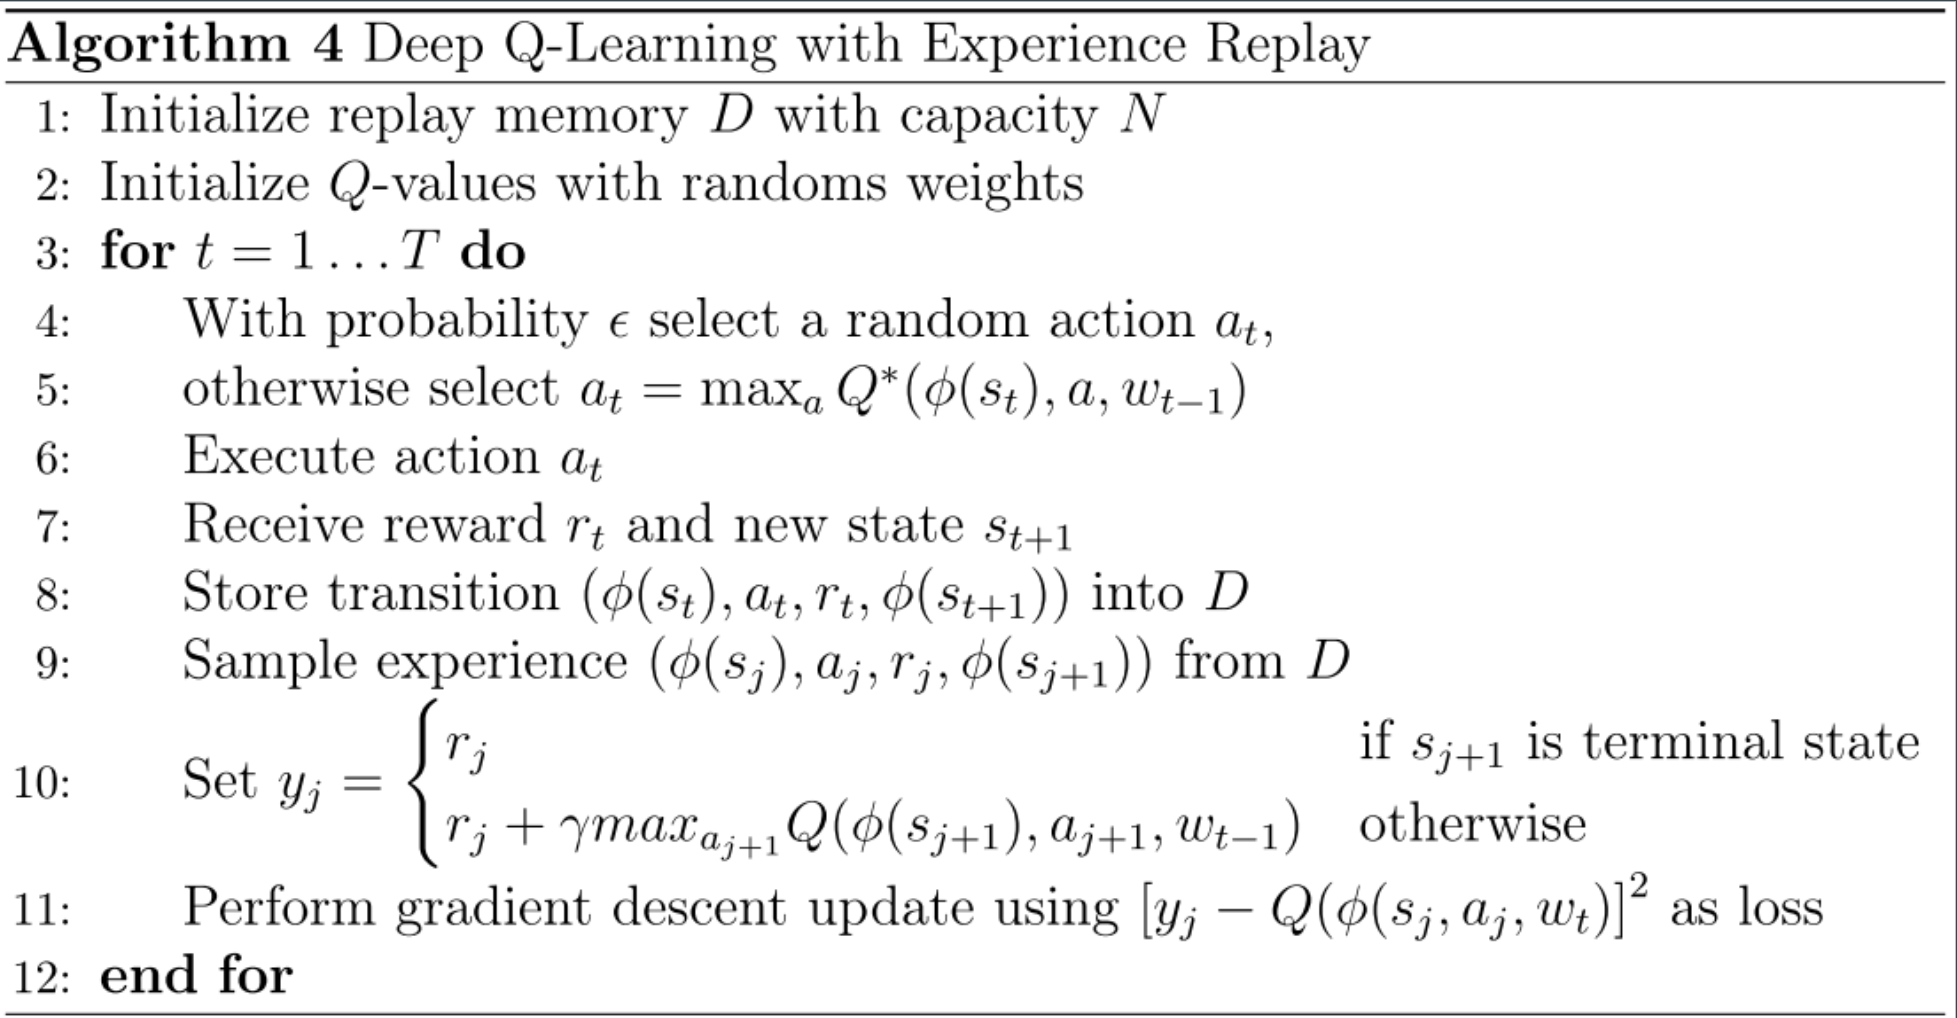
\includegraphics[width=0.65\textwidth]{images/alg.png}
        \caption{ Deep Q-Learning algorithm }
      \label{fig:compare}
      \caption{}
   \end{figure}

\section{Results}
To tackle this project, there were lots of iterations that was needed in order to create a proper model environemtn and for it 
to achieve our desired objectives. At first, the initial parameters were used to simulate and run the environment but adding a negative reward at the end 
of the episode. At the end, our test cases showed the HGV to glide in a really flat trajectory and then descends down 
relatively fast. This seemed like what we initially wanted but from the data, it can be seen that it ended the episode 
early at around 1/10 of the original downrange using a constant angle of attack. 

Due to the performance of the trajectory for the heading angle, thoughts on if the issue was more on the neural net was done. 
The episodes was increased to 1000 from 100, the gamma changed from 0.7 to 0.85 to highlight the importance of future actions so it doesn't try to crash earlier. 
Lastly due to the increase in episode number, the minibatch was increased to 64. After doing all of these changes, the effect on the trajectories 
was still the same so the focus changed not on the neural network but on the rewards structure.

With the same effect but much higher number of episodes, the number of episodes was greatly decreaed to 100 again. At the same time, the gamma was increased to 0.95.
To reward going higher distances, an extra reward of the downrange was added while also penalizing if the terminating downrange was below 1000km. This had better results,
and incremental improvements was desired.

In order to address this, splits in the exploration, training and testing were done. To have a bigger source of memory for training, the exploration was increased to 35\% of the episodes, 
while training account for 65\% of the episodes. At the same time, some limitations were removed which was now just the altitude because a low velocity eventually gets a low altitude soon anyway. 
The number of episodes was increased to 250 with a minibatch of 32 as well. There were some further explorations with our rewards structure by being more lenient with the heading angle 
so an absolute value was used instead. 

Lastly, due to a recent collaboration and ideation, adding generality for the controller would be great so there were now different initial conditions added so the state space may be greatly increased.
At the same time, extra limitations were added due to the physical representatio of the model. This should have been added earlier but was disregarded for the sake of exploration. 

We now summarize the runs of the DNN Q-learning. Two of our runs are listed Figure \ref{fig:training_data_plots}. 
We see consistency that between the two figures, as the network progresses in training, the algorithm 
learns slowly to keep the heading angle near zero while maximizing range. Its evident by subfigure 
\ref{fig:run_3} that it has developed a policy for incentivizing max range. This is supported by the 
early failed regions in subfigure \ref{fig:run_2} where the trajectories did not exceed 1,000 km 
in down range distance. 

\begin{figure}[H]
   \begin{subfigure}[b]{0.5\textwidth}
     \centering
     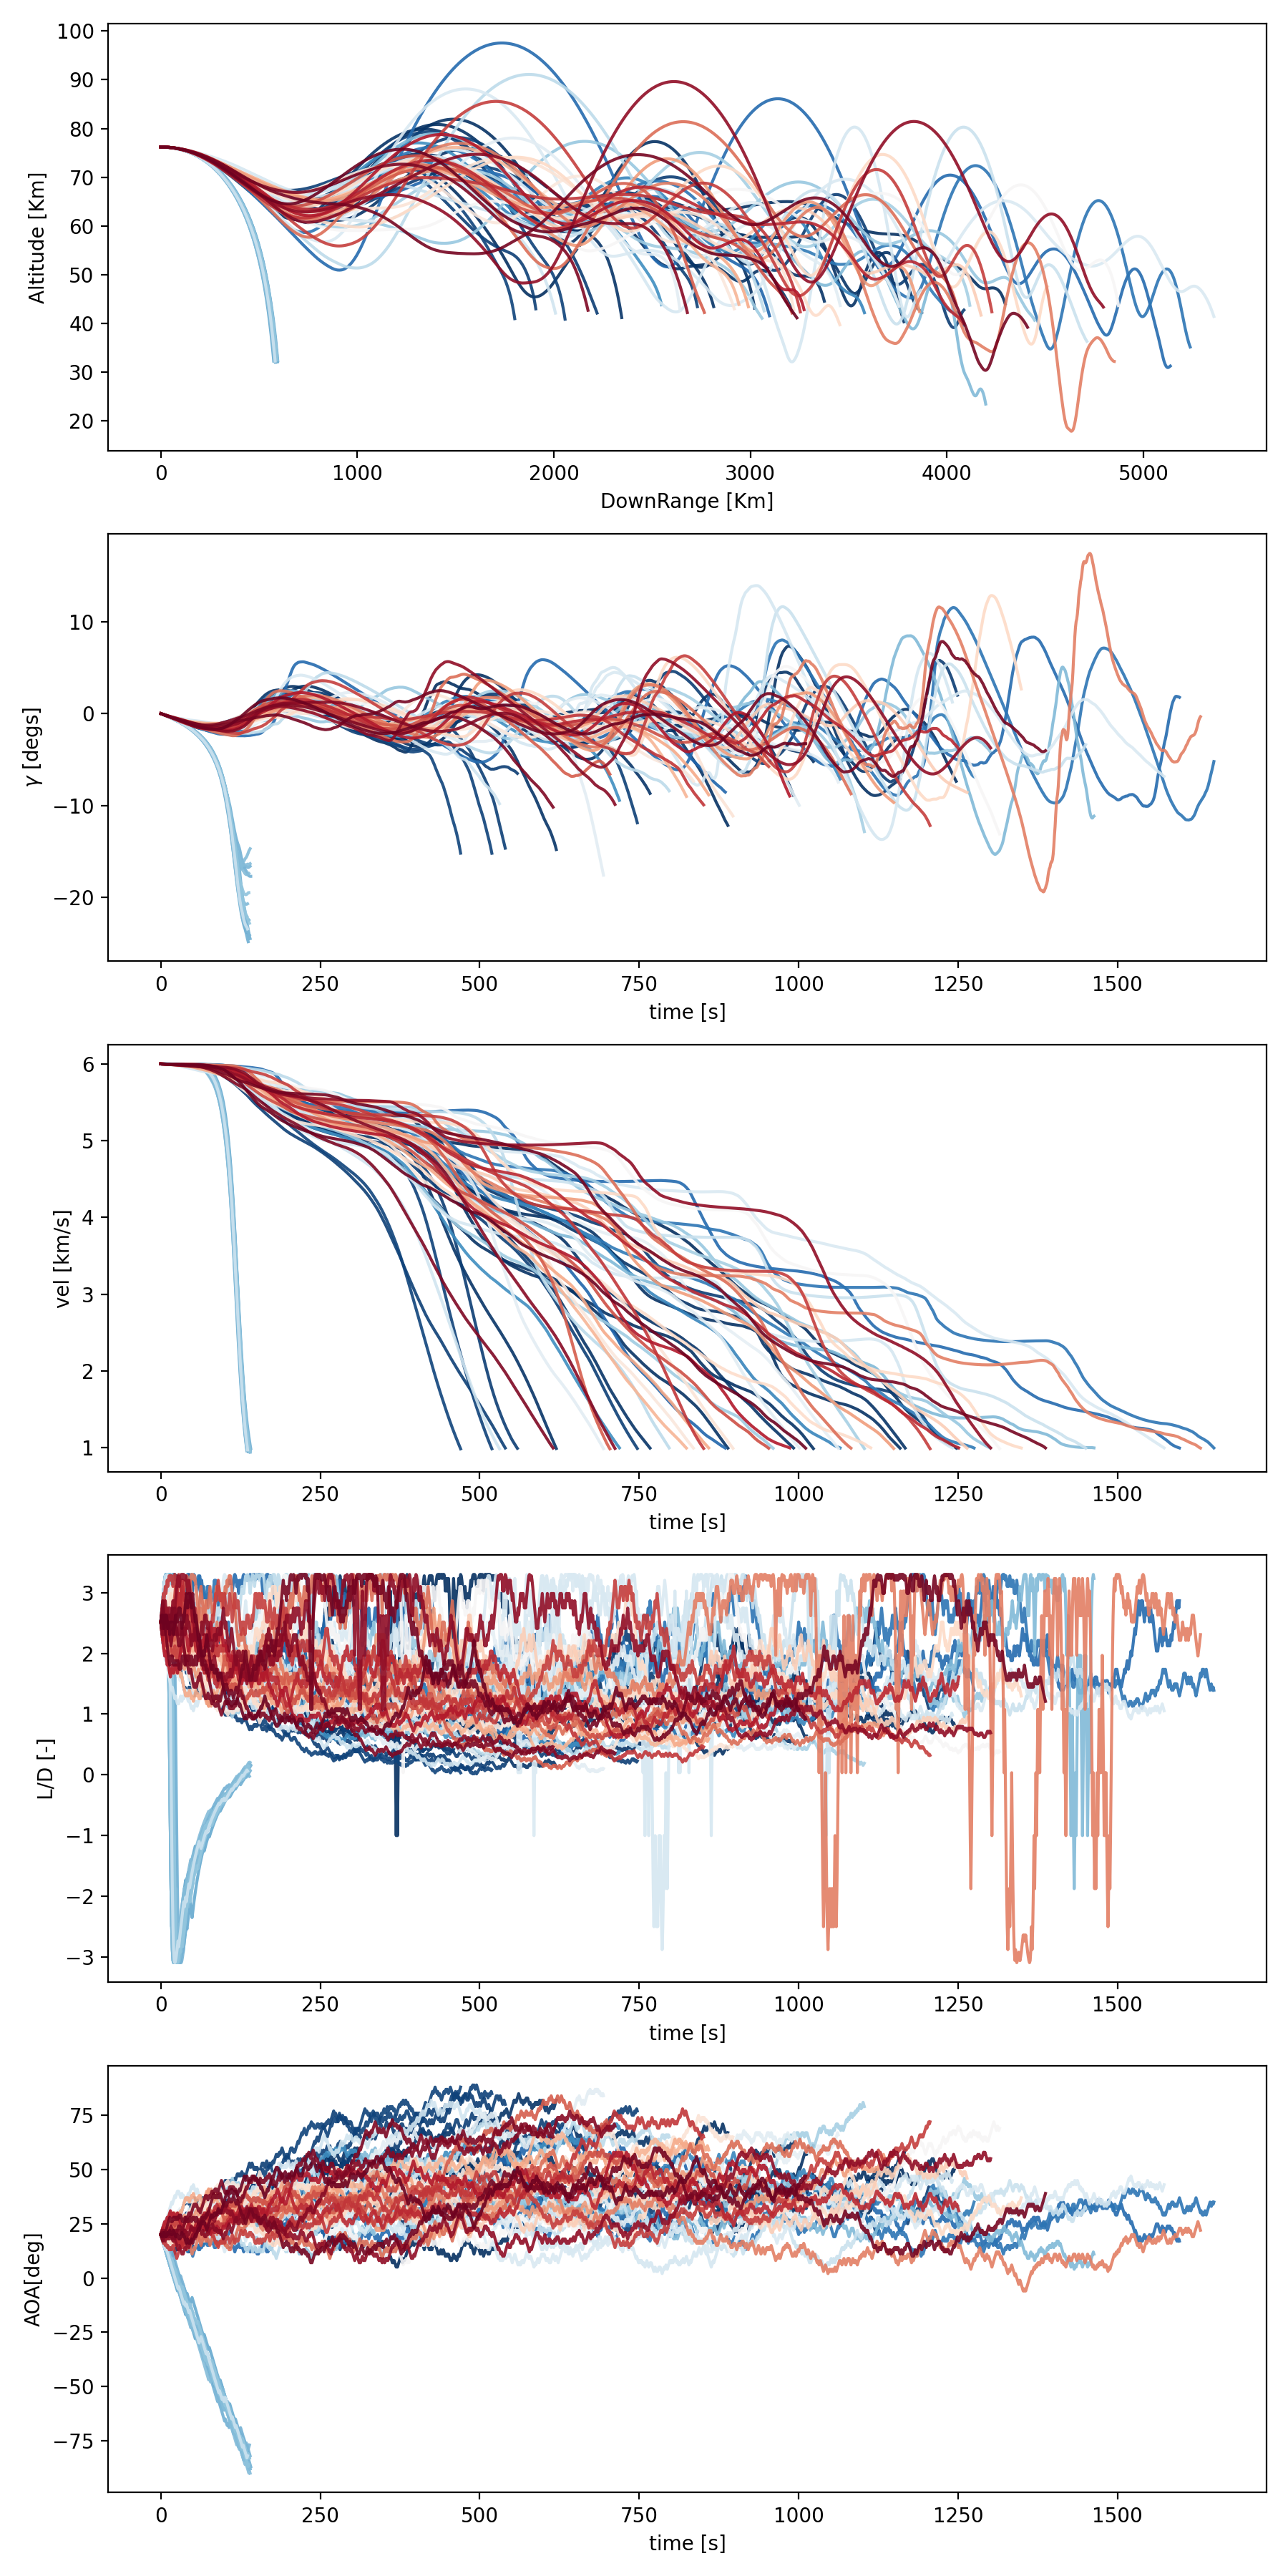
\includegraphics[width=\textwidth]{images/run_2.png}
     \caption{ Run 2}
     \label{fig:run_2}

   \end{subfigure}
   \begin{subfigure}[b]{0.5\textwidth}
     \centering
     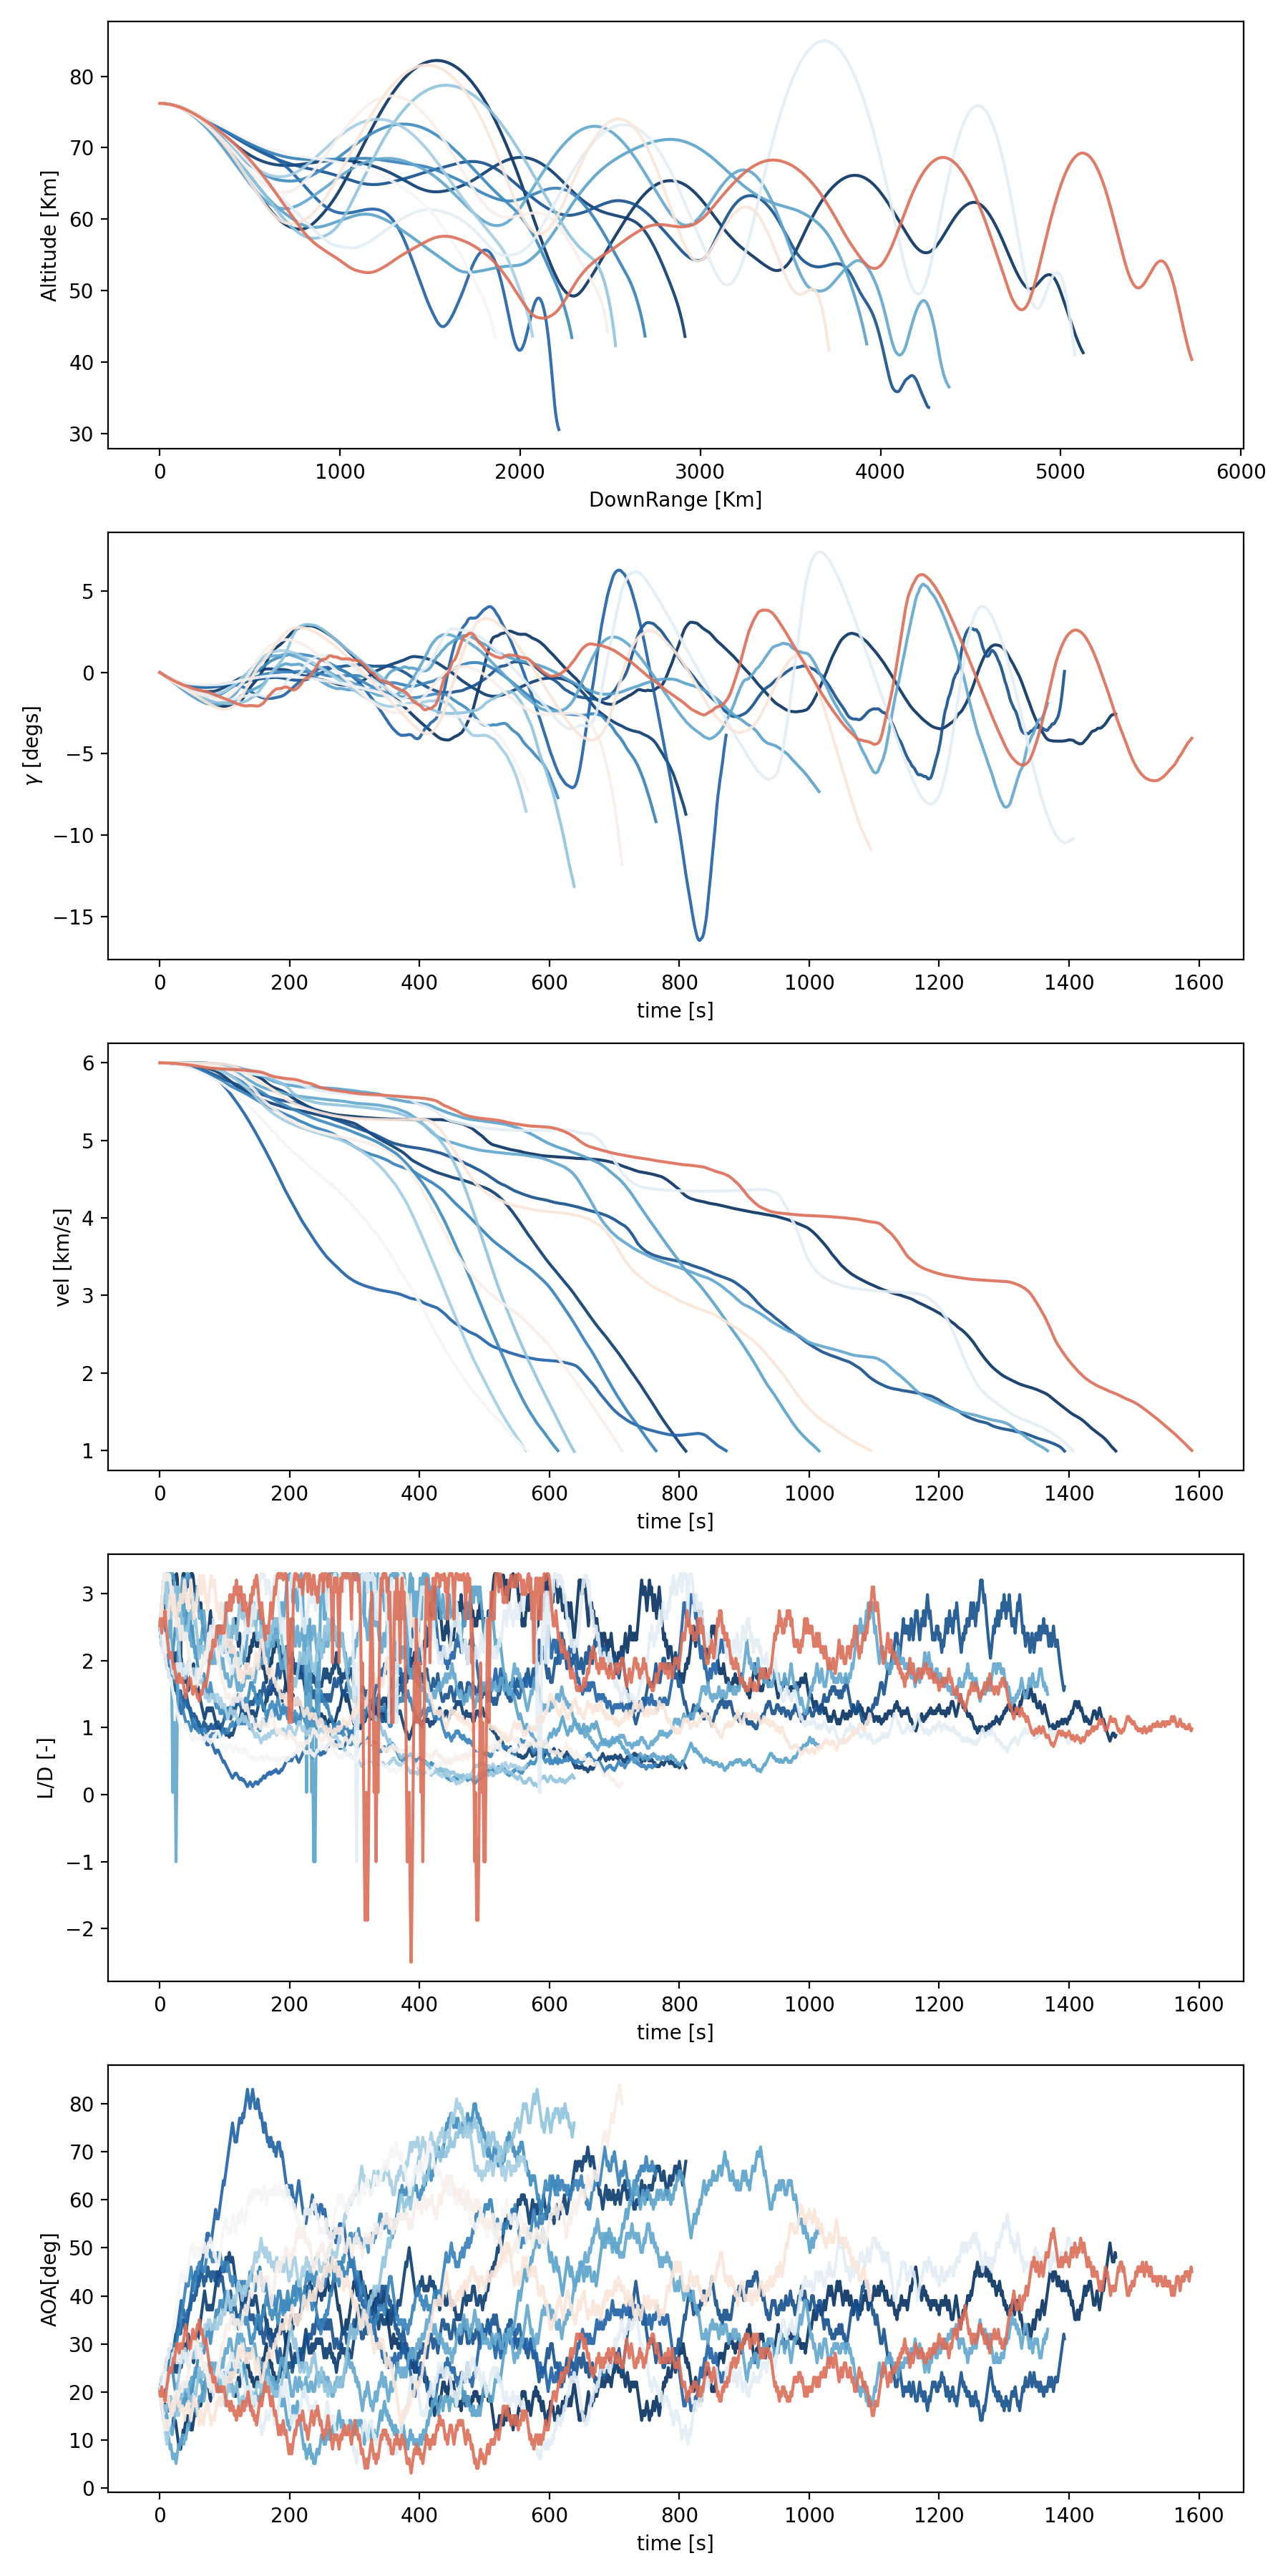
\includegraphics[width=\textwidth]{images/run_3.png}
     \caption{ Run 3}
     \label{fig:run_3}

   \end{subfigure}
   \caption{Output runs of DNN Q-learning. Blue signifies earlier portions of the training while red signifies later in training}
   \label{fig:training_data_plots}

\end{figure}
When we implement the policy after updating the results of two runs are shown in Figure \ref{fig:run_data_plots}. 
We see that the policy performance is acceptable for the earlier portions of the trajectory. However, as expected,
once velocities are lower more lift is needed to maintain level fligth. Hence, we see notable trends upward 
in subfigure \ref{fig:run_81}. We see in subfigure \ref{fig:run_82} just how sensitive initial chooses effect 
guidance for the policy. We note this by the subtle decrease in subfigure \ref{fig:run_81} as opposed to 
the increase in \ref{fig:run_82} leading to very different angle of attack progression but similar trajectory
profiles in altitudes.

\begin{figure}[H]
   \begin{subfigure}[b]{0.5\textwidth}
     \centering
     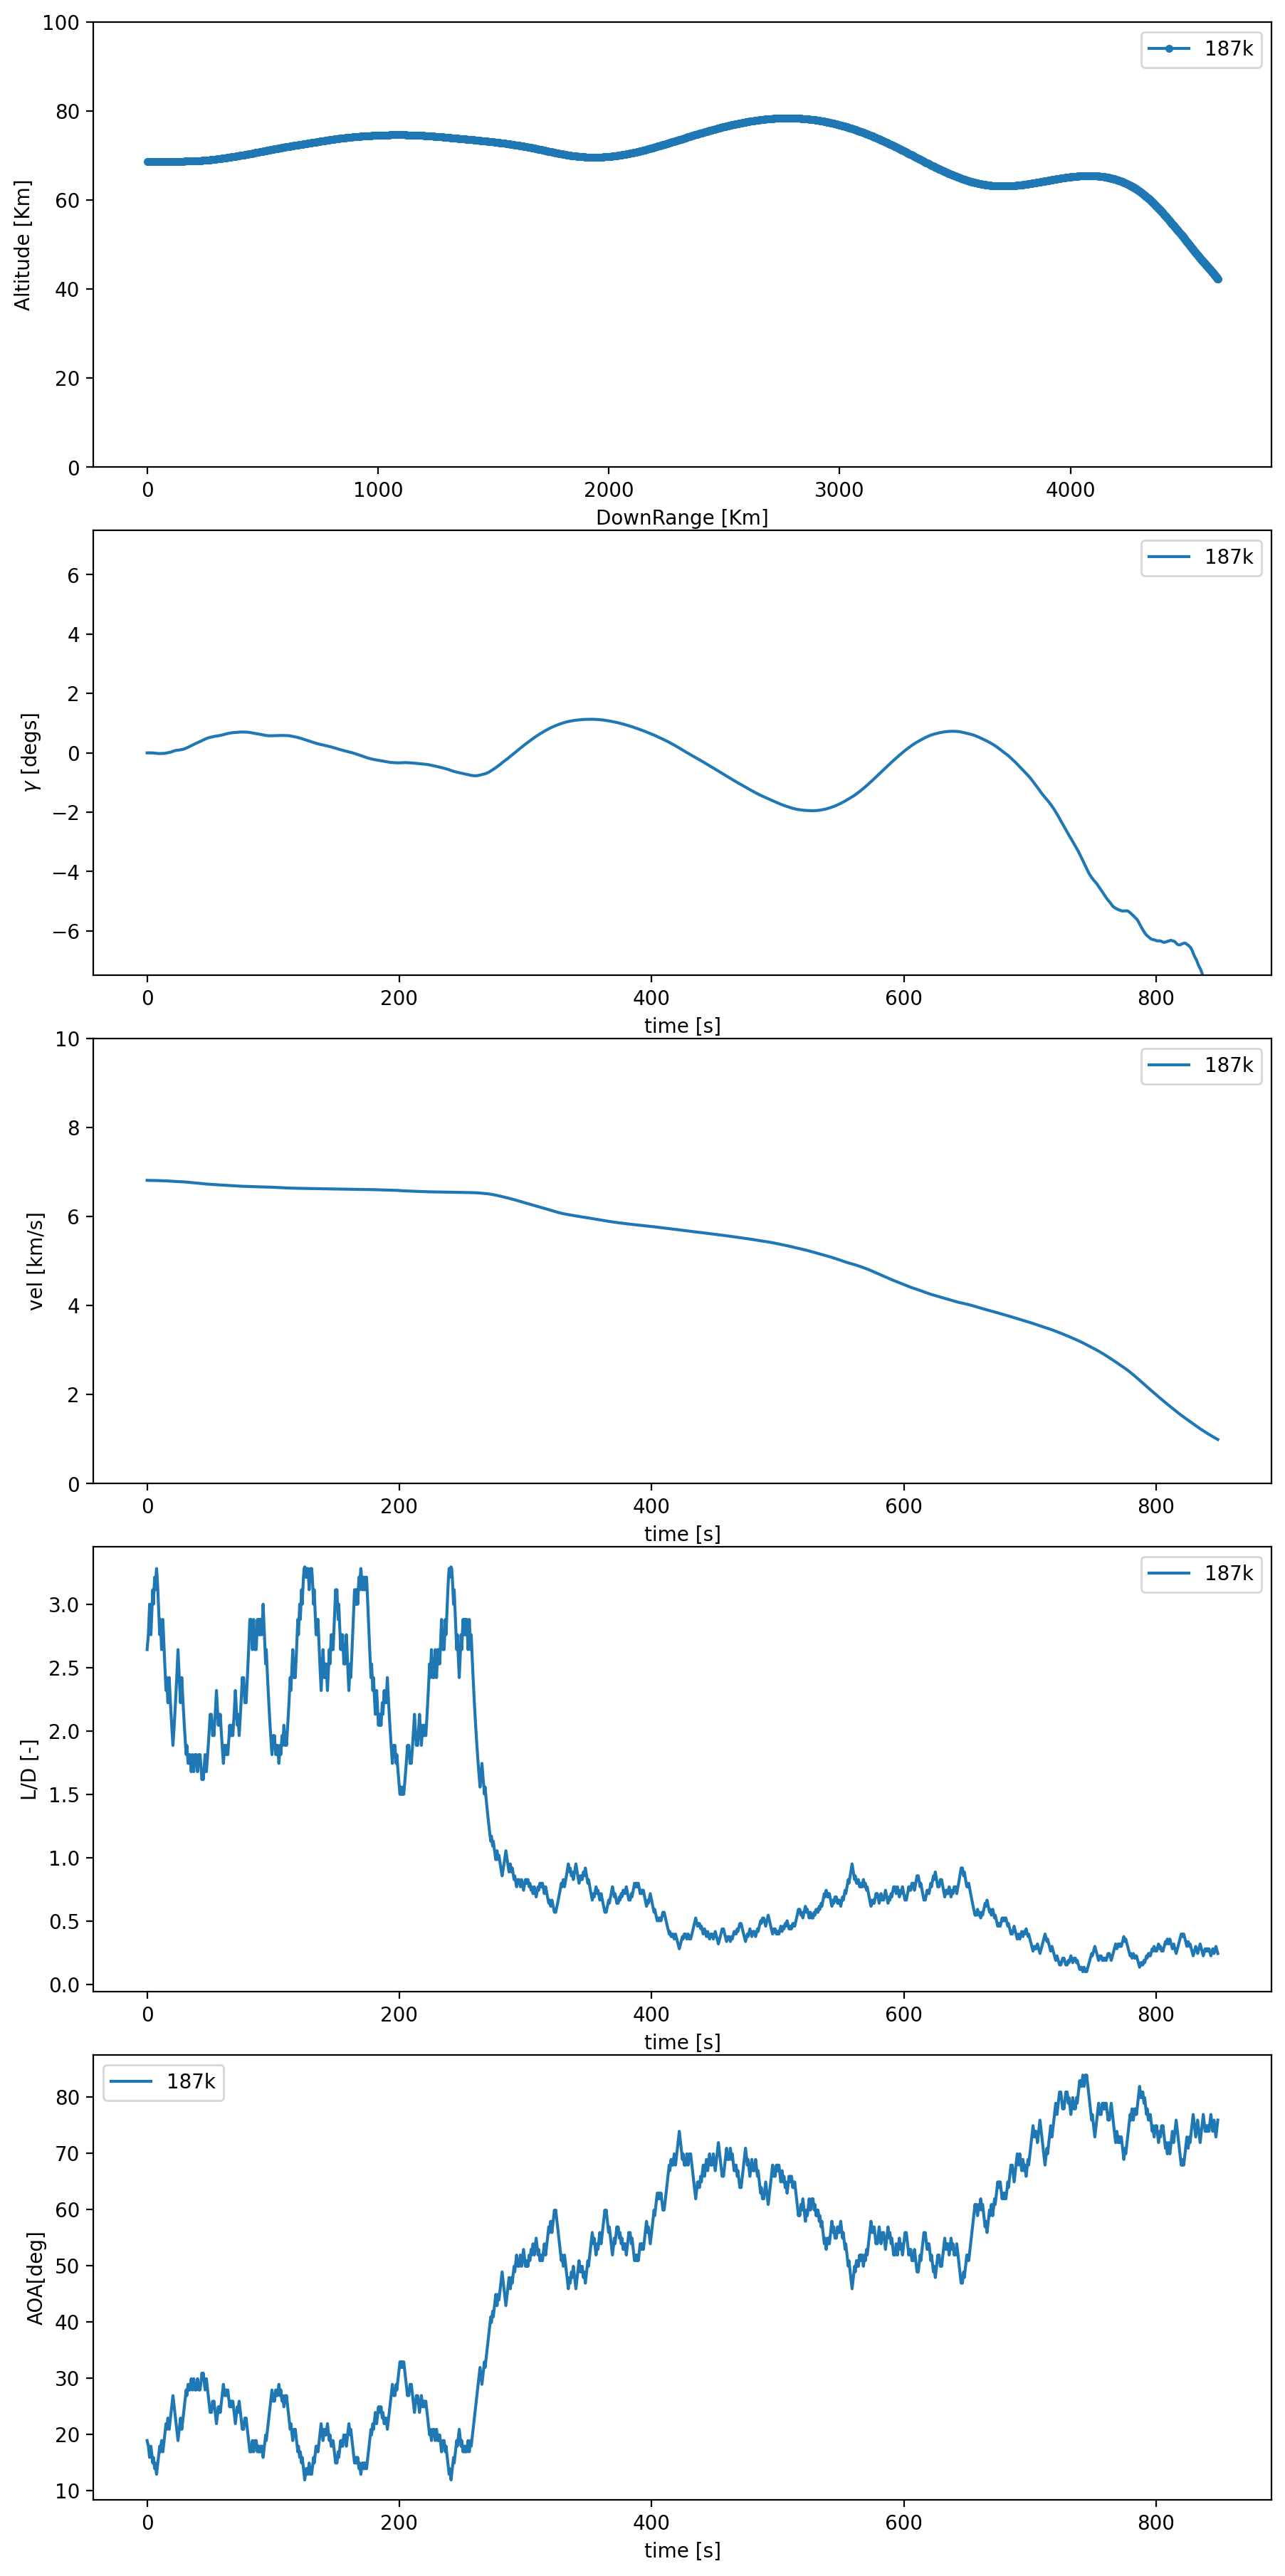
\includegraphics[width=\textwidth]{images/run8_explore.png}
     \caption{Testing optimal policy run 1}  
     \label{fig:run_81}
   \end{subfigure}
   \begin{subfigure}[b]{0.5\textwidth}
     \centering
     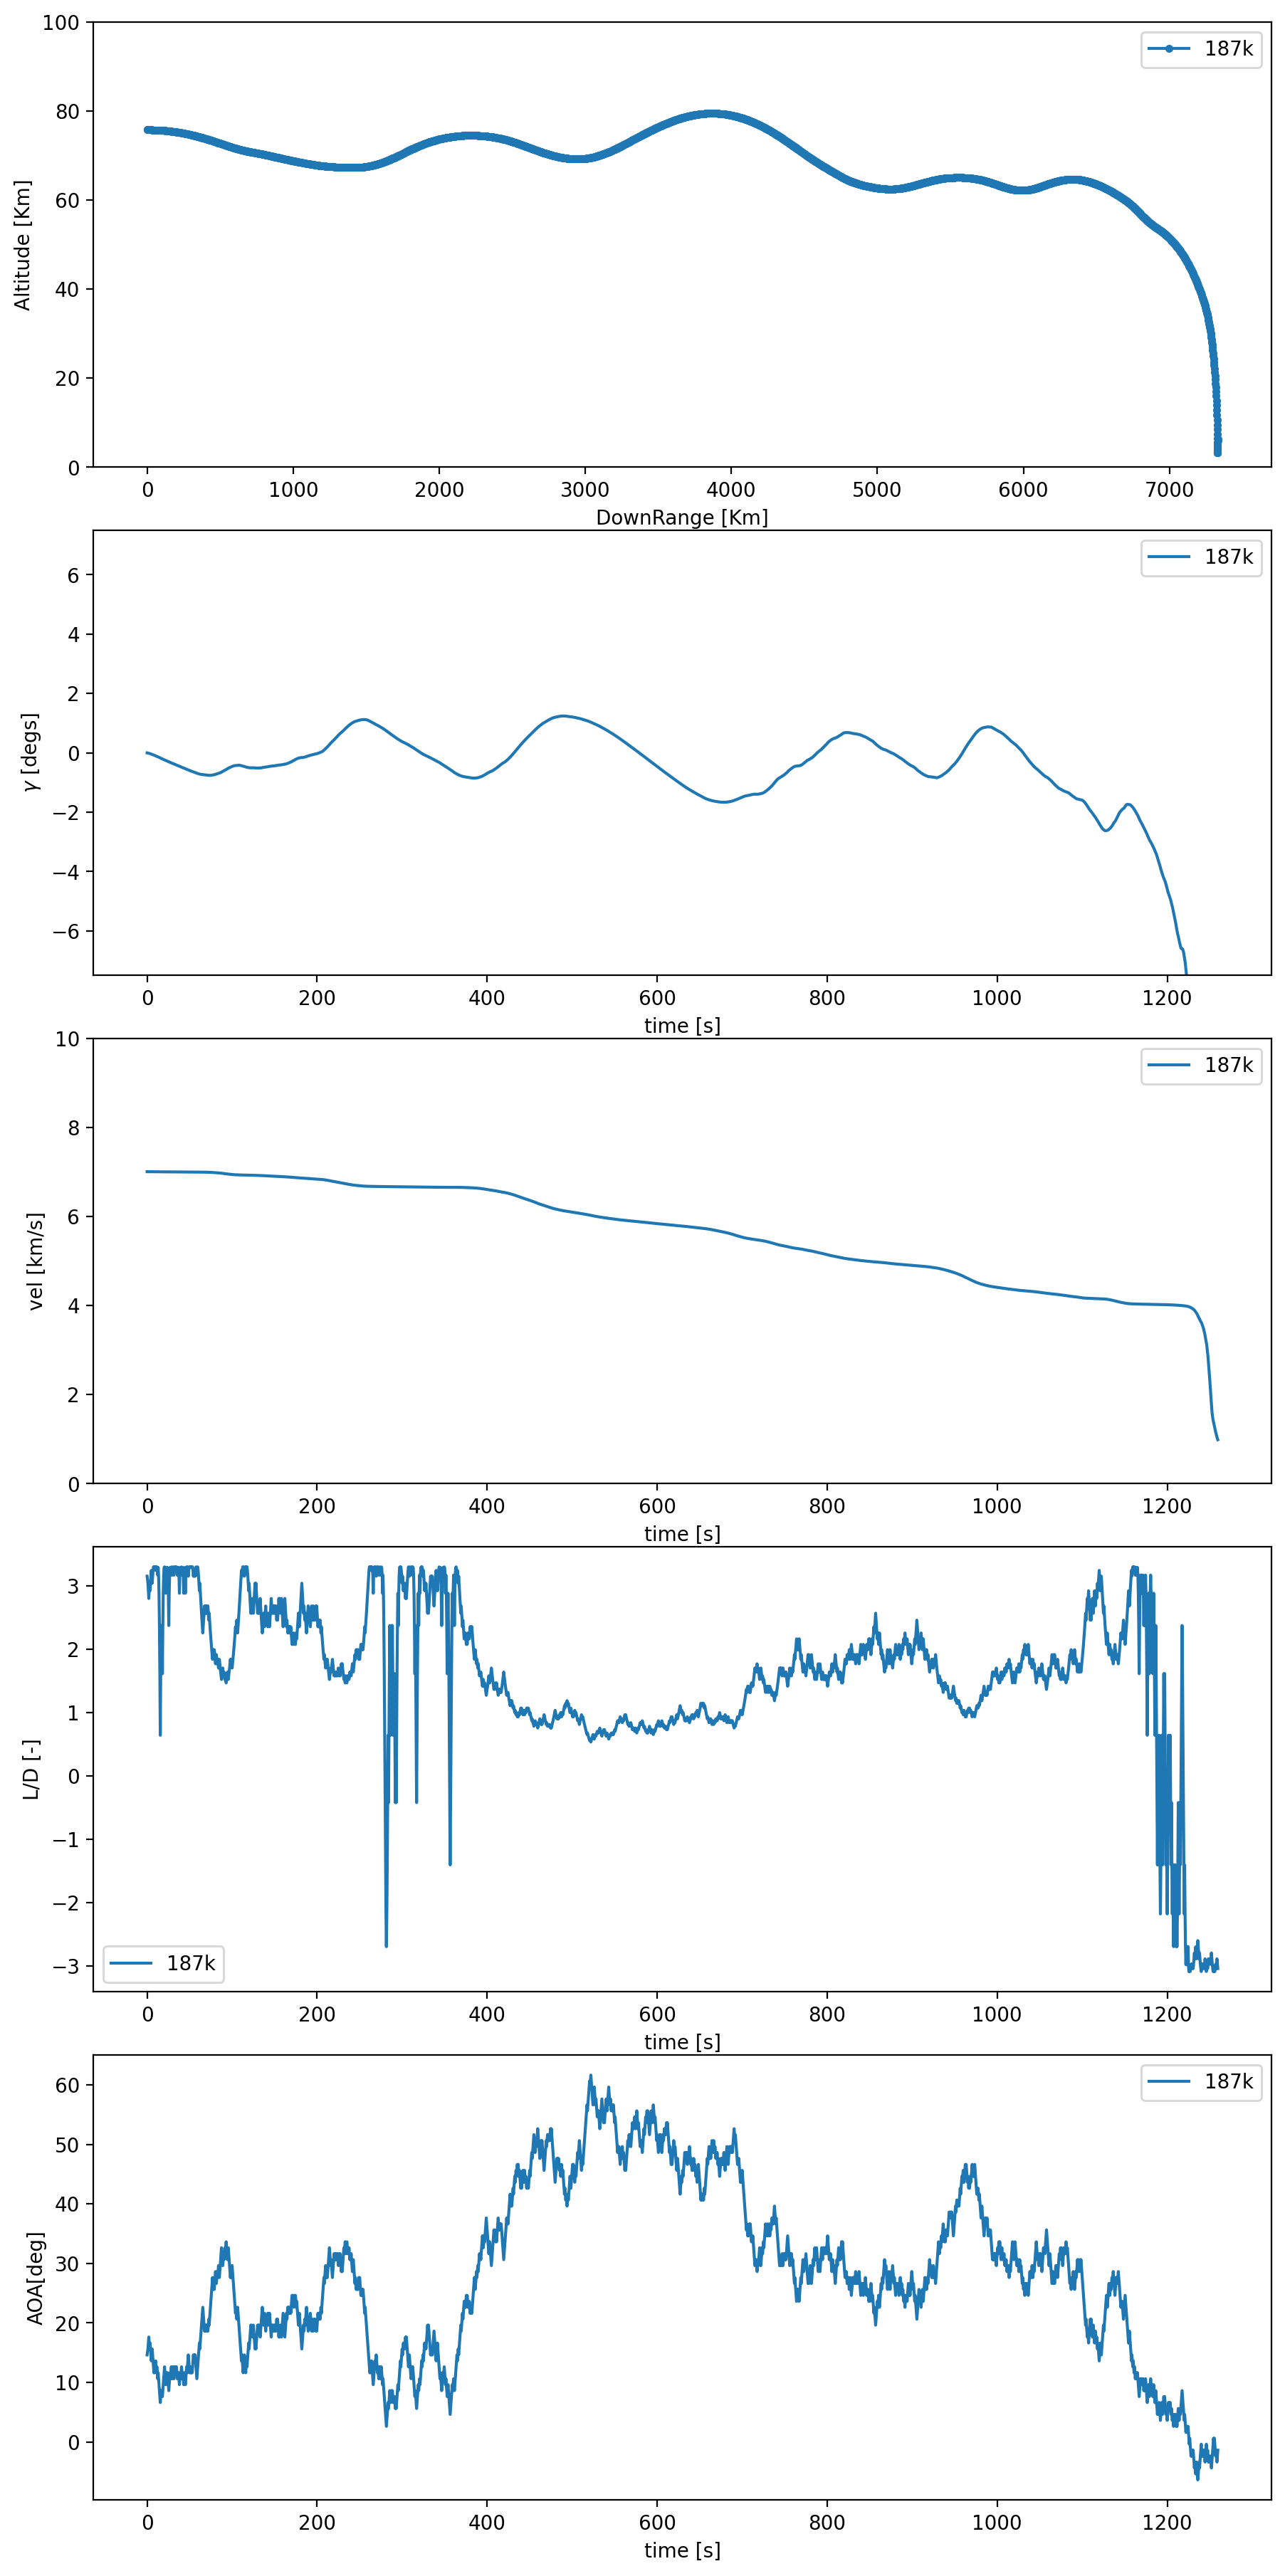
\includegraphics[width=\textwidth]{images/run8_explore2.png}
     \caption{ Testing optimal policy run 2}
     \label{fig:run_82}

   \end{subfigure}

   \caption{Online run of $\pi*$ after training}
   \label{fig:run_data_plots}

\end{figure}
\section{Discussion}
Compared with other MDP problems, this is more complex due to the usage of the ODE and there is no analytical solution 
for the controls problem. However, we have showed a new approach for simulating and controlling a hypersonic glide vehicle using simplified physics
and reinforment learning. Some of the key insights that we have discovered while doing this project is that firstly, Choosing a suitable neural network 
architecture for the policy and value functions was not trivial, as different architectures had different trade-offs in terms of complexity, 
performance, and generalization. We experimented with various architectures and compared their results to find the best one for our problem. Additionally, we have experienced that
uning the hyperparameters of the neural network and the reinforcement learning algorithm was also a difficult task, as they affected the convergence, stability, and robustness 
of the learning process. We used a trial-and-error approach and followed some best practices to find the optimal values for the hyperparameters.

We would report that our main issue was designing a proper reward function which was crucial for achieving our objective of maintaining a flat heading angle. 
We found that different reward functions had different impacts on the final output, and that some reward functions did not encourage the desired behavior. 
We also had to consider the trade-off between accuracy and computation time, as higher accuracy required more computation time and vice versa.

Some key limitations include the number of episodes that the model was trained on, even if it was then modeled to be generalizable for any initial condition. At the same time,
we also had difficulty in balancing multiple goals, such as minimizing the heading angle but also not having it to terminate too early. Afterwards, due to the scope of the simplified physics
it terminates early after the altitude reaches a high height. Qualitatively, this trajectory is good because there was not that much reduction in velocity while also having a straight heading angle.
Unfortunately, this better controls can't be used or it won't be physically intuitive. In the end, we had to settle but something mediocre but was still able to perform better than the constant angle-of-attack.

\section{Conclusions}
In conclusion, we have showed the feasibility of using a neural net for reinforcement 
learning of a hypersonic glide vehicle. This was achieved by running multiple episodes and was split into an exploration, 
training, and testing state. In the exploration stage, the action taken was completely random, while in the training stage, 
the randomness of the action choosing was slowly decreasing. With our goal of having a flat heading angle, the new trajectory 
of the HGV is much different than the constant angle of attack case. There were lots of issues that was faced during the 
simulation for each run because of the limitations on some of the state space values so it is still physically representative 
and accurate. Overall, in addition with training hyperparameters, this was addressed by changing the rewards, termination 
and neural net hyperparameters. And was able to get a proper control system using the first few timesteps of the gliding. 

For future work, extended training time and a more complex neural network architecture may train the controller better 
to fit our objectives more accurately. A neural network generally gets more complex with various combinations of sequential 
blocks and activation functions as the model to be trained gets more complicated. In this case, with a 3 layer fully connected layer, 
this is definitely not enough as the number of nodes cannot fully represent a complex 4 state ordinary differential equation. Different work
in the realm of machine learning has been done with the use of LSTMs or Residual Blocks which add complexity. Additionally, it can be noted that
neural networks have a tendency to overfit the data so the use of dropout layers may benefit the model.

\newpage
\section*{Appendix}
\subsection*{ Trajectories with constant angle-of-attack }
\begin{figure}[hbt!]
    \begin{subfigure}[b]{0.5\textwidth}
      \centering
      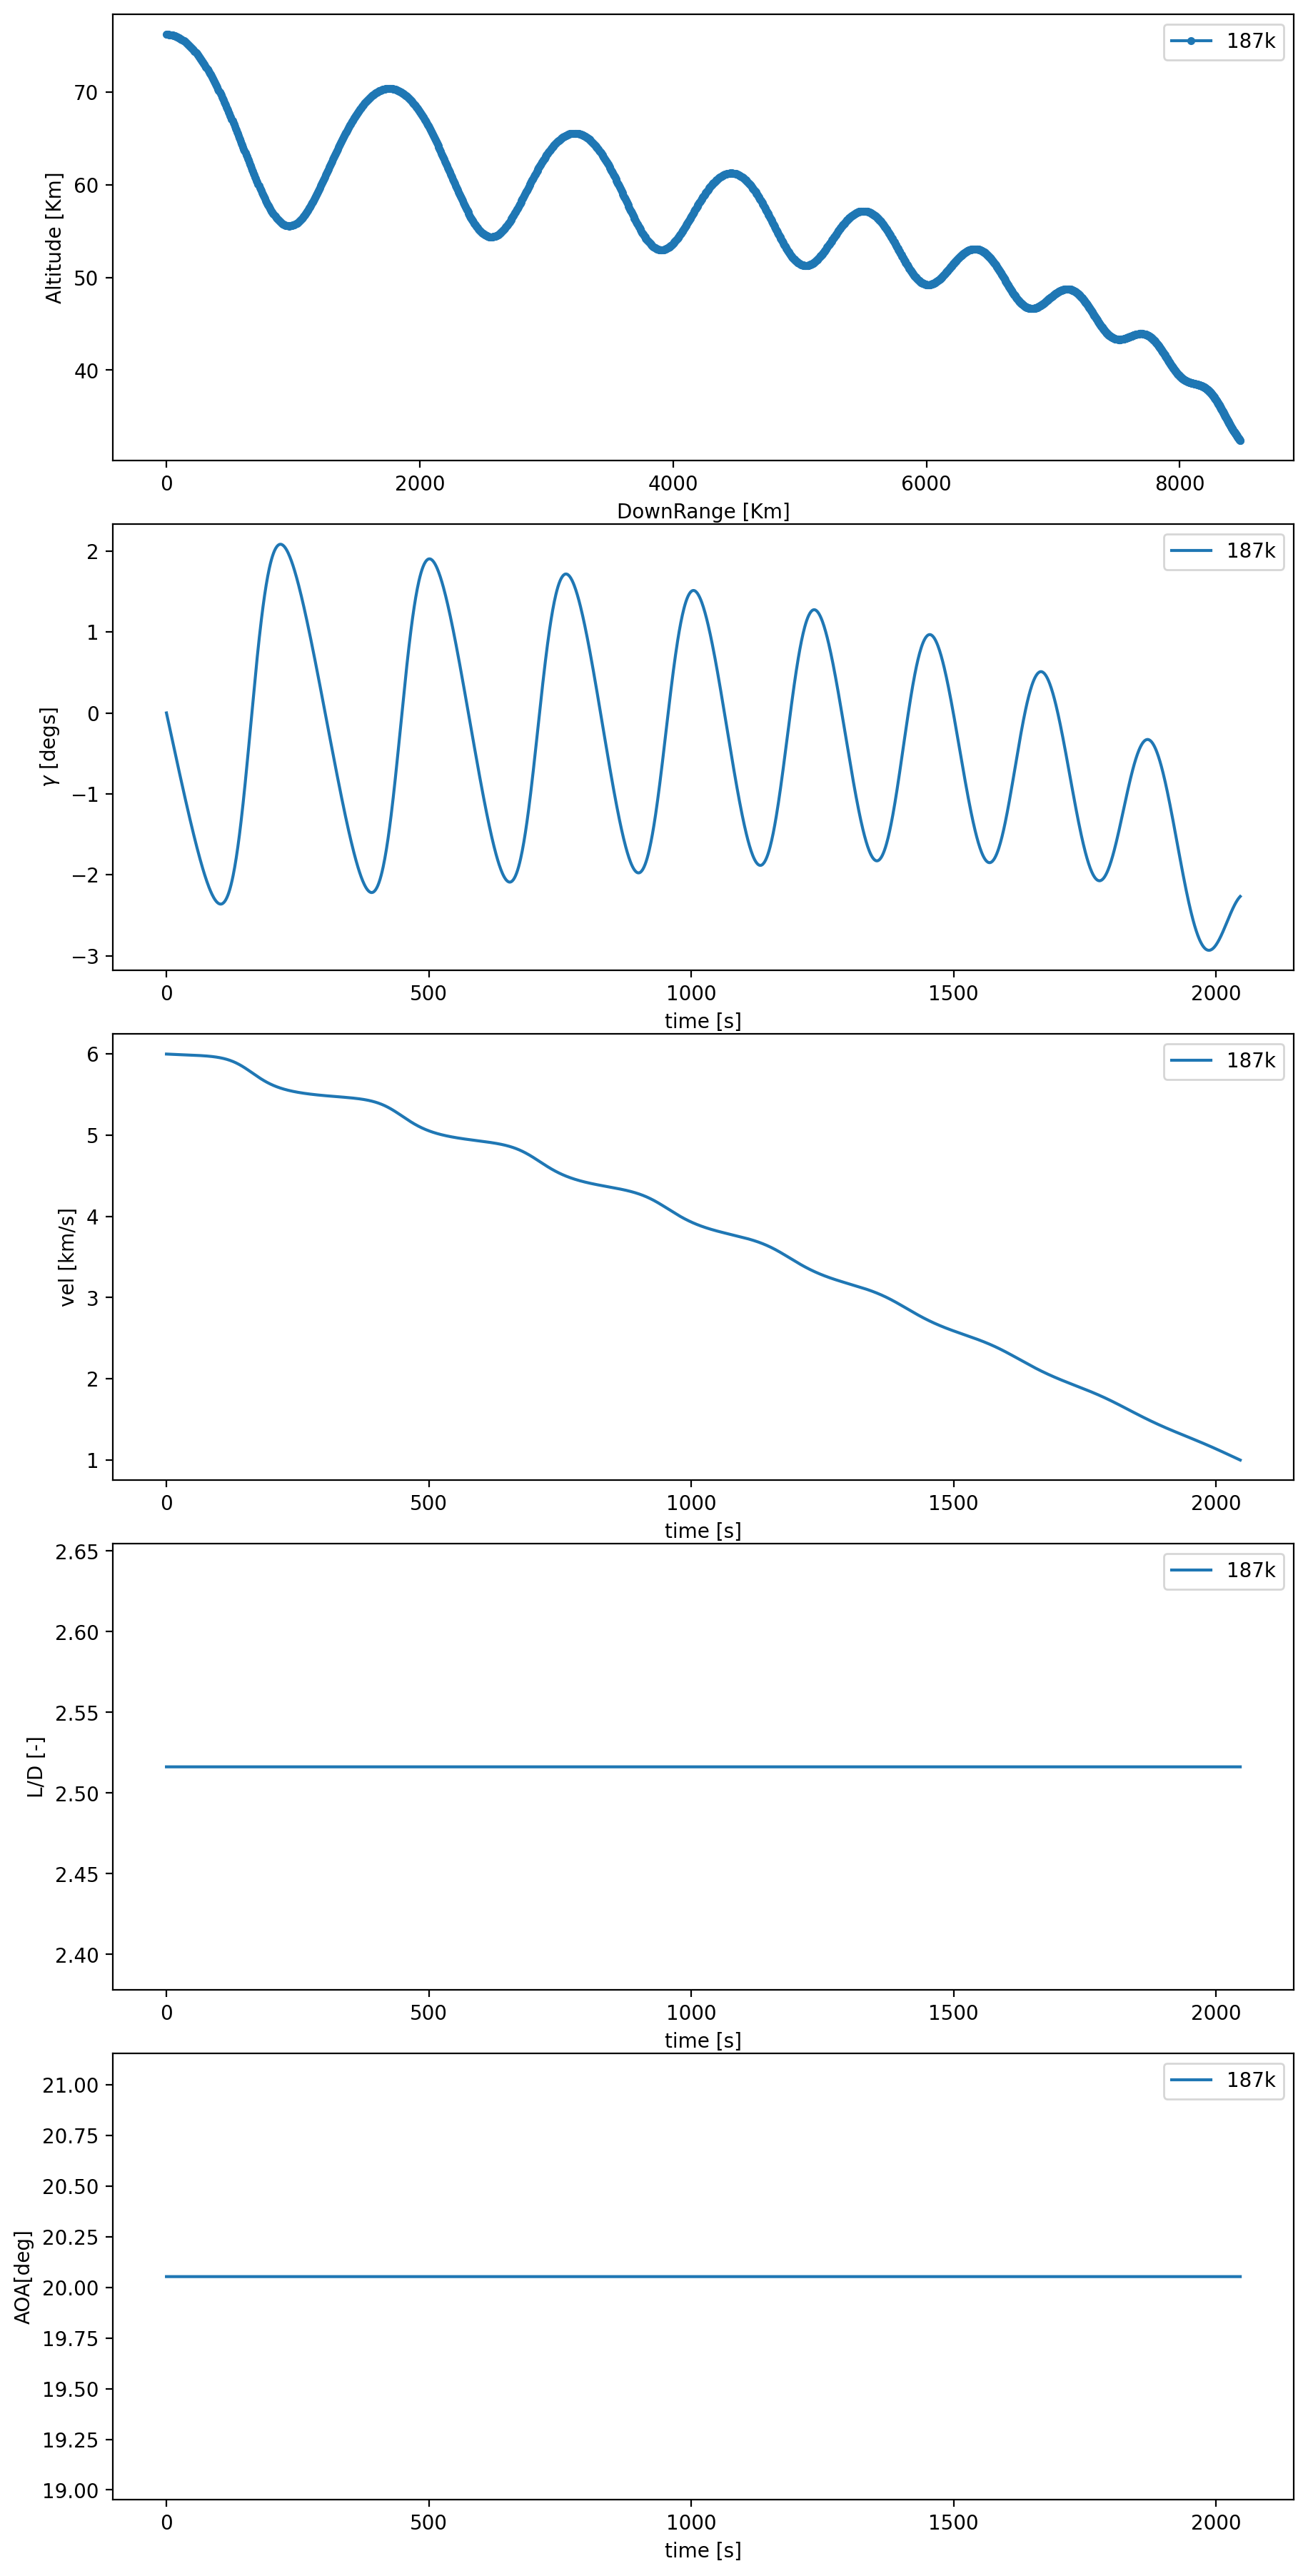
\includegraphics[width=\textwidth]{images/og1.png}
      \caption{ vel = 6km/s,  alt=76.2 km,   $\alpha$=20.05}
    \end{subfigure}
    \begin{subfigure}[b]{0.5\textwidth}
      \centering
      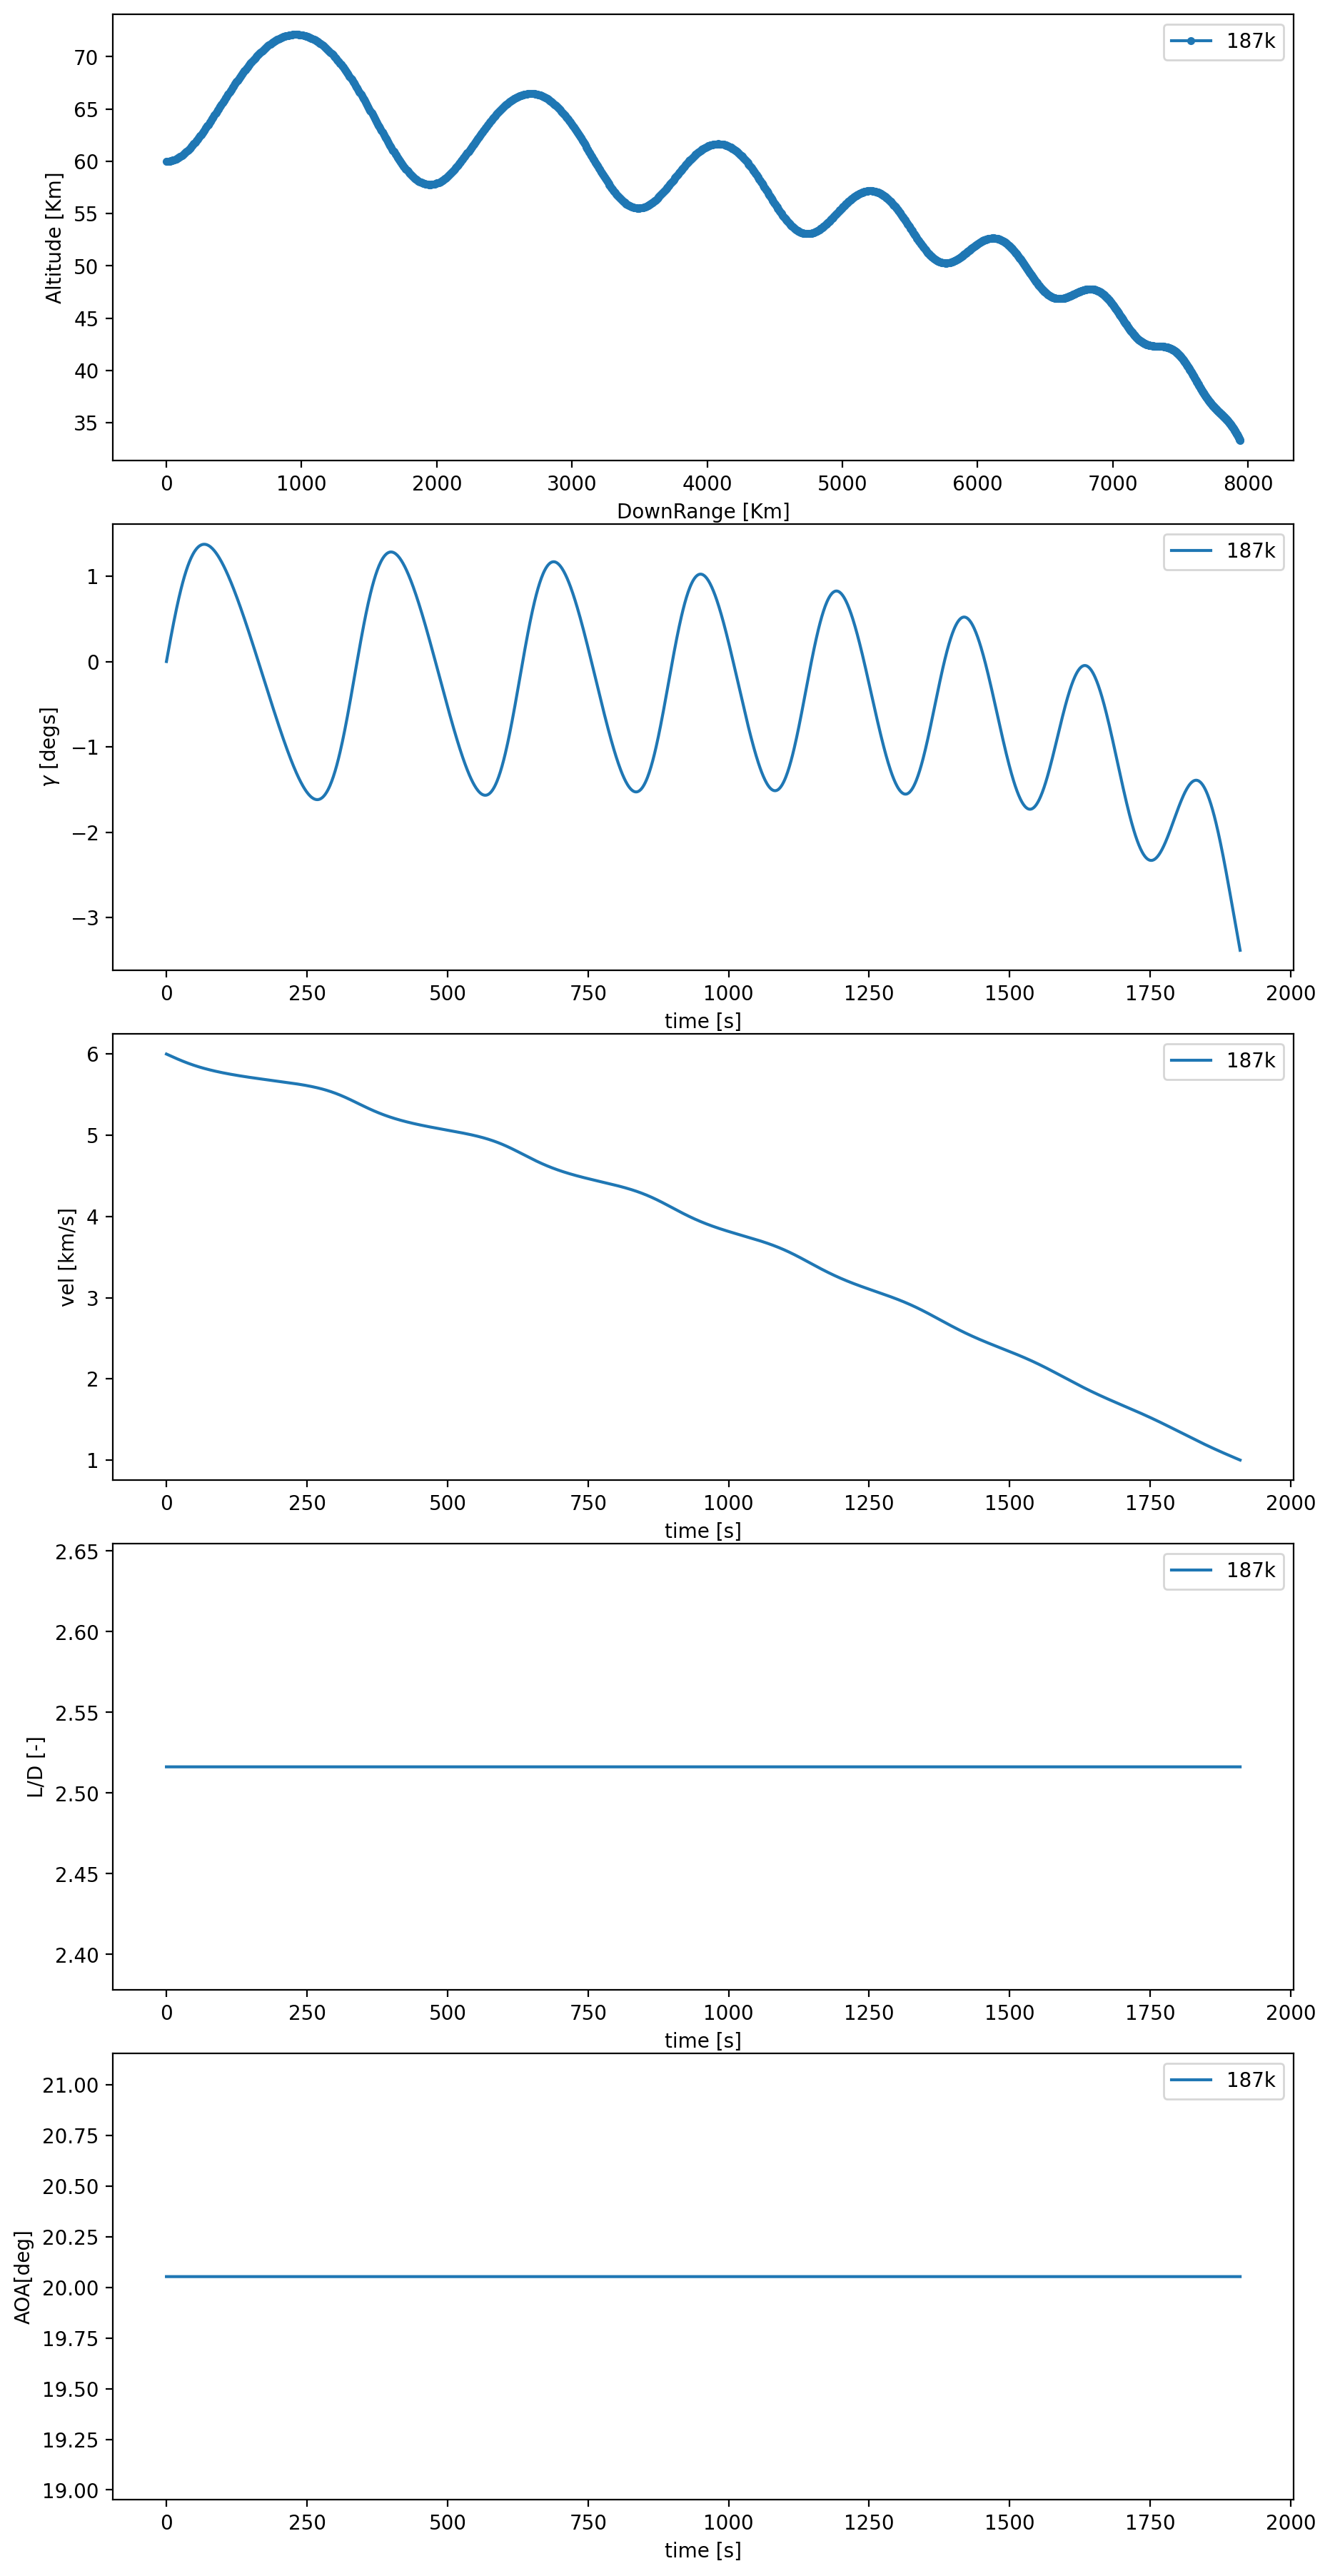
\includegraphics[width=\textwidth]{images/og2.png}
      \caption{ vel = 6km/s,  alt=60.0 km,   $\alpha$=20.05}
    \end{subfigure}
\end{figure}

\newpage
\subsection*{ Hypersonic Glide Vehicle Environment }
\lstset{style=mystyle}
\lstinputlisting[language=Python]{code/sim_NeuralNet.py}

\newpage
\subsection*{ Neural Network with Deep Q-Learning }
\lstset{style=mystyle}
\lstinputlisting[language=Python]{code/NeuralNet_jj.py}

\end{document}
